\documentclass[12pt]{article}
%\RequirePackage{amsthm,amsmath,amsfonts,amssymb}
\RequirePackage[colorlinks,linkcolor=cyan,citecolor=red,urlcolor=magenta]{hyperref}
\RequirePackage{fix-cm}

\usepackage[table,xcdraw]{xcolor}
\usepackage{arydshln}
\usepackage{color,soul}
\usepackage{accents,float,graphicx,subfig,multirow,dcolumn,booktabs,lscape}
\usepackage{comment}
\usepackage[letterpaper,margin=0.9in]{geometry}
\usepackage[ruled,linesnumbered]{algorithm2e}
\usepackage[font=normal]{caption}
\usepackage[title]{appendix}

%thick cdot
\makeatletter
\newcommand*\bigcdot{\mathpalette\bigcdot@{.5}}
\newcommand*\bigcdot@[2]{\mathbin{\vcenter{\hbox{\scalebox{#2}{$\m@th#1\bullet$}}}}}
\makeatother

\newcommand{\size}[2]{{\fontsize{#1}{0}\selectfont#2}}
\newenvironment{sizepar}[2]
 {\par\fontsize{#1}{#2}\selectfont}
 {\par}

\SetAlFnt{\small}

\pagestyle{myheadings}

%eqn, def numbering
\numberwithin{equation}{section}

\theoremstyle{definition}
\newtheorem{definition}{\protect\definitionname}
\providecommand{\definitionname}{Definition}
\numberwithin{definition}{section}

\theoremstyle{plain}
\newtheorem{lemma}{\protect\lemmaname}
\providecommand{\lemmaname}{Lemma}
\numberwithin{lemma}{section}

\theoremstyle{plain}
\newtheorem{theorem}{\protect\theoremname}
\providecommand{\theoremname}{Theorem}
\numberwithin{theorem}{section}

\newcommand{\appendixpagenumbering}{
  \break
  \pagenumbering{arabic}
  \renewcommand{\thepage}{\thesection-\arabic{page}}
}

% highlighting
\newcommand{\hlgreen}[2][green]{{\sethlcolor{#1}\hl{#2}}}
\newcommand{\hlning}[2][orange]{{\sethlcolor{#1}\hl{#2}}}

\newcommand{\ind}{\perp\!\!\!\!\perp}
\newcommand{\ts}{\rlap{$^{***}$}}
\newcommand{\ds}{\rlap{$^{**}$}}
\newcommand{\s}{\rlap{$^{*}$}}

\def\spacingset#1{\renewcommand{\baselinestretch}{#1}\small\normalsize}\spacingset{1}

\newcolumntype{.}{D{.}{.}{-1}}

% path for figures
\graphicspath{{figures/}}

% Remove irritating PDFLaTeX warnings
%\pdfminorversion=6
\pdfminorversion=7
\pdfsuppresswarningpagegroup=1

\RequirePackage{amsthm,amsmath,amsfonts,amssymb}
\RequirePackage[colorlinks,linkcolor=cyan,citecolor=red,urlcolor=magenta]{hyperref}
\RequirePackage{fix-cm}

\usepackage[table,xcdraw]{xcolor}
\usepackage{arydshln}
\usepackage{color,soul}
\usepackage{accents,float,graphicx,subfig,multirow,dcolumn,booktabs,lscape}
\usepackage{comment}
\usepackage[letterpaper,margin=0.9in]{geometry}
\usepackage[ruled,linesnumbered]{algorithm2e}
\usepackage[font=normal]{caption}
\usepackage[title]{appendix}

%thick cdot
\makeatletter
\newcommand*\bigcdot{\mathpalette\bigcdot@{.5}}
\newcommand*\bigcdot@[2]{\mathbin{\vcenter{\hbox{\scalebox{#2}{$\m@th#1\bullet$}}}}}
\makeatother

\newcommand{\size}[2]{{\fontsize{#1}{0}\selectfont#2}}
\newenvironment{sizepar}[2]
 {\par\fontsize{#1}{#2}\selectfont}
 {\par}

\SetAlFnt{\small}

\pagestyle{myheadings}

%eqn, def numbering
\numberwithin{equation}{section}

\theoremstyle{definition}
\newtheorem{definition}{\protect\definitionname}
\providecommand{\definitionname}{Definition}
\numberwithin{definition}{section}

\theoremstyle{plain}
\newtheorem{lemma}{\protect\lemmaname}
\providecommand{\lemmaname}{Lemma}
\numberwithin{lemma}{section}

\theoremstyle{plain}
\newtheorem{theorem}{\protect\theoremname}
\providecommand{\theoremname}{Theorem}
\numberwithin{theorem}{section}

\newcommand{\appendixpagenumbering}{
  \break
  \pagenumbering{arabic}
  \renewcommand{\thepage}{\thesection-\arabic{page}}
}

% highlighting
\newcommand{\hlgreen}[2][green]{{\sethlcolor{#1}\hl{#2}}}
\newcommand{\hlning}[2][orange]{{\sethlcolor{#1}\hl{#2}}}

\newcommand{\ind}{\perp\!\!\!\!\perp}
\newcommand{\ts}{\rlap{$^{***}$}}
\newcommand{\ds}{\rlap{$^{**}$}}
\newcommand{\s}{\rlap{$^{*}$}}

\def\spacingset#1{\renewcommand{\baselinestretch}{#1}\small\normalsize}\spacingset{1}

\newcolumntype{.}{D{.}{.}{-1}}

% path for figures
\graphicspath{{figures/}}

% Remove irritating PDFLaTeX warnings
%\pdfminorversion=6
\pdfminorversion=7
\pdfsuppresswarningpagegroup=1


%dark mode
\pagecolor[rgb]{0.1,0.1,0.1} %shallow black
\color[rgb]{0.85,0.85,0.85}  %shallow grey

%%%%%%%%%%%%%%%%%%%%%%%%%%%
%%%%%%%%%%%%%%%%%%%%%%%%%%%
%%%%%%%%%%%%%%%%%%%%%%%%%%%

\begin{document}

\pagenumbering{gobble}

\title{\bf Solar: a least-angle regression of stable and ultrafast variable selection for high dimensional and large-scale data}
\author{Ning Xu \hspace{.4cm}\\
  Timothy C.G. Fisher \hspace{.4cm}\\
  and \hspace{.4cm}\\
  Jian Hong \hspace{.4cm}\\
  School of Economics, University of Sydney \hspace{.4cm}\\
  NSW, Australia, 2006}
\clearpage\maketitle

\begin{abstract}
  %
  We propose a new algorithm for variable selection for high-dimensional, large-scale data, called \emph{subsample-ordered least-angle regression (solar)} and its coordinate-descent generalization. Solar relies on the average $L_0$ solution path computed across subsamples and alleviates several high-dimensional issues with lasso, strong/safe rule, variable ranking methods and subsampling-based variable selection. We illustrate in simulations that, with the same computation load, solar yields substantial improvements over lasso in terms of the sparsity (37-64\% reduction in the average number of selected variables), stability and accuracy of variable selection. Our example shows that, compared with strong/safe rule and variable screening, solar largely rectifies the incorrect variable purge at complicated dependence structures. Moreover, solar supplemented with the hold-out average test(a new adaptation of the data-splitting hypothesis test) successfully purges almost all of the redundant variables while retaining all of the informative variables. Using simulations and real-world data, we also illustrate numerically that sparse solar variable selection is robust to complicated dependence structures and harsh settings of the irrepresentable condition. Moreover, replacing lasso with solar in a subsampling-based variable selection algorithm (e.g., the bootstrap lasso or stability selection), significantly reduces the computation load (at least 96\% fewer subsample repetitions) and improves selection sparsity. Using Python interface and Intel Math Kernel Library, We provide a Fortran/C++ based parallel computing package for solar (\texttt{solarpy}) in both the supplementary file and \href{https://github.com/isaac2math/solar}{dedicated Github page}.
  %
\end{abstract}

\noindent
\normalsize
Keywords: lasso sparsity, multicollinearity, irrepresentable condition, bolasso, stability selection, variable ranking

\vfill
\newpage
\spacingset{1.4} 

%%%%%%%%%%%%%%%%%%%%%%%%%%%%%%%
%%%%%%%% INTRODUCTION  %%%%%%%%
%%%%%%%%%%%%%%%%%%%%%%%%%%%%%%%

\clearpage
\pagenumbering{arabic}

\section{Introduction}

In the last decade, lasso-related algorithms have been widely applied to high dimensional, large-scale applications. Various improvements have been proposed, including \citet{zou2005regularization}, \citet{zou2006adaptive} and \citet{friedman10}. However, the improvements often come at the cost of a higher computation load, making lasso-related algorithms less attractive at large-scale applications like computer vision and natural language processing (typically with $p$ at millions and data at GBs). Optimization of the lasso-type tuning parameter is often combined with cross validation (CV), further increasing the computation load in complex models \citep{xu2012asymptotic}. \citet{lim2016estimation} shows that CV-based lasso-type estimators may lead to models that are unstable in high dimensions and consequently ill-suited for interpretation and generalization. Thus, in a world of ever-expanding data size, it remains an ongoing challenge to improve the variable-selection performance of lasso-type estimators while restraining the computation load.

Least-angle regression \citep{efronall04, friedman2010regularization}, alongside with coordinate descent \citep{friedman2007pathwise}, imbues lasso-type estimators with ultra-fast computation. However, research shows that lasso may still be sensitive to sampling randomness, complicated dependence structures, noise and outliers in high-dimensional spaces \citep{weisberg04,lim2016estimation}. Furthermore, higher data dimensions are often associated with more severe multicollinearity and more complicated dependence structures, compelling variable-selection algorithms to utilize as much relevant finite-sample information as possible to enhance the accuracy, stability and robustness of variable-selection. To alleviate such issue, subsampling variable selection (e.g., \citet{bach2008bolasso}, \citet{meinshausen2010stability}) have been proposed to improve the variable-selection accuracy and stability of CV-lasso. Given CV-based lasso merges the computation loads of lasso and CV, repeating CV-based lasso many times magnifies computation load, particularly less attractive in large-scale applications and reproducing kernel Hilbert spaces. Another approach is to conduct post-lasso selection, e.g., the `safe rule' \citep{ghaoui2010safe} or the `strong rule' \citep{tibshirani2012strong}. However, both rules may incorrectly purge informative variables or repeatedly propose modifications \citep{wang2014safe, zeng2017efficient}. In contrast to lasso, variable screening (aka unconditional correlation ranking) \citep{fan2008sure, li2012feature, li2012robust} ranks variables by absolute values of their unconditional correlations to $Y$ and selects the top $w$ variables based on CV, bootstrap or BIC. Lastly, to conduct the classical hypothesis tests after selection, \citet{wasserman2009high}, \citet{meinshausen2009p} and \citet{barber2019knockoff} propose the data split scheme. The orginal data is split, reserving one part for selection and the other for testing. However, such method depends on the split scheme and may result in efficiency loss due to testing on only a fraction of the data.

\subsection{Motivating examples}
%
We illustrate the variable selection accuracy and stability issues in high-dimensional data using two well-known examples from the literature. Example~1 shows that lasso may have a variable-selection stability problem due to its $L_1$ arc. Example~2 shows that lasso may have a variable-selection accuracy issue when the dependence structure is complicated.

\smallskip
\noindent
\textbf{Example 1.} \citep{lim2016estimation} To reduce computation load, the lars-lasso algorithm (i.e., lasso solved by the lars algorithm) uses the $L_1$-norm ratio $t \in [0, 1]$ as a tuning parameter to control shrinkage, where $t = 0$ corresponds to shrinking all $\beta_i$ to $0$ and $t = 1$ corresponds to no shrinkage. In each CV training-validation split, $\forall\beta$ on the solution path, $t = \left\Vert \beta \right\Vert_1 / \left\Vert \beta_{\mathrm{max}} \right\Vert_1$ where the denominator is the $L_1$ norm of the non-shrinked solution. \citet{lim2016estimation} show that the solution path of lars-lasso is unstable in high dimensions. When $p > n$, $\beta_{\mathrm{max}}$ is the traditional forward regression solution with $n$ selected variables, which uses up all $n$ degrees of freedom (a saturated fit), implying, due to the resampling randomness in CV, that $\left\Vert \beta_{\mathrm{max}} \right\Vert_1$ may vary substantially across validation sets. As a result, the same value of $t$ may correspond to different amounts of shrinkage on the solution paths of different CV training-validation splits, limiting the usefulness of $t$ and adversely impacting selection accuracy and stability. Coordinate descent suffers a similar problem since, when $p>>n$, the $\lambda$ grid $\left\{ \lambda_{min}, \lambda_{max} \right\}$ may be significantly different across subsamples. The larger $(p - n)$, the more severe the problems. $\blacksquare$

\smallskip
\noindent
\textbf{Example 2.} \citep{zhaoyu06} Consider the following dependence structure
%
\begin{equation}
            %
            \begin{cases}
            %
    \mathbf{x}_3 = \omega \mathbf{x}_1 + \omega \mathbf{x}_2 + \sqrt{1 - 2 \omega^2} \cdot u \\
    %
    Y = \beta_1 \mathbf{x}_1 + \beta_2 \mathbf{x}_2 + \delta e \\
    %
            \end{cases}
            %
            \label{eqn:example_2}
            %
\end{equation}
%
where the $\mathbf{x}_i$ are standardized; $e$ and $u$ are independent Gaussian noises; $\delta$, $\omega$, $\beta_1$ and $\beta_2$ are scalars. Since only $\mathbf{x}_1$ and $\mathbf{x}_2$ are informative variables for $Y$, an accurate algorithm should select only $\mathbf{x}_1$ and $\mathbf{x}_2$. The irrepresentable condition (IRC) is fundamental for variable selection accuracy in lasso and forward regression. Whether IRC is satisfied in this case depends on the values of $\omega$, $\beta_1$ and $\beta_2$. In simulations with $\delta = 1$, $\omega = \textstyle\frac{2}{3}$, $\beta_2 = 3$ and $n = 1,000$, strong IRC fails when $\beta_1 = 2$ while IRC holds when $\beta_1 = -2$. When IRC fails, lars-lasso wrongly selects $\mathrm{x}_3$ as an informative variable of $Y$; when strong IRC holds, the mistake is avoided. The challenge in this example is the high correlation between $\mathbf{x}_3$ and the informative variables, examples of which may be pervasive in the complicated dependence structures of empirical data. Since multicollinearity may violate IRC and induce errors in variable selection, the robustness of selection algorithms to multicollinearity and complicated dependence structures is an important empirical issue. $\blacksquare$

The challenge in Example~2 is the strong multicollinearity, which may be pervasive in the complicated dependence structures of empirical research. Strong multicollinearity may violate IRC and induce errors into variable selection. Thus, the robustness of variable selection to strong multicollinearity and complicated dependence structures is an important empirical issue.

\subsection{Main results}

In this paper, we propose a new algorithm for variable selection in high-dimensional data, called  \emph{subsample-ordered least-angle regression} (solar). Solar is based on the average $L_0$ solution path from least-angle regression or coordinate descent on multiple subsamples. With the same computation load as lasso, alleviates several known high-dimensional issues with lasso, strong/safe rule, variable ranking methods and subsampling-based variable selection. Further, solar is robust to complicated dependence structures in regression analysis and is potentially generalizable to variable selection with a variety of lasso-type and forward regression estimators.

Using simulations, we demonstrate the following attributes of solar: (1) when $p/n$ approaches $0$ or $1$, with the same computation load as lasso, solar is more responsive to changes in $p/n$, yielding significant improvements in variable-selection performance over lasso; (2) when $n$ and $p$ both increase rapidly in high-dimensional space, solar significantly outperforms lasso in terms of convergence tendency, sparsity (a 37-64\% reduction in the average number of selected variables), stability and accuracy of variable selection; (3) in our simulation, supplementing solar with the hold-out average test (a new adaptation of the data-splitting test) successfully purges almost all of the redundant variables while retaining all of the informative variables; (4) compared with safe/strong rule and variable screening, our examples show that solar is robust to non-standard dependence structures in regression analysis, implying better variable-selection accuracy under different settings of the IRC; (5) replacing lasso with solar in the subsampling-based variable selection algorithms largely removes redundant variables from the ranking, resulting in a significant computation load reduction (at least 96\% fewer subsample repetitions) and a improvement on selection sparsity and accuracy.

The paper is organized as follows. In section~\ref{section:algo}, we introduce solar and its coordinate descent generalization. In section~\ref{section:adv} and \ref{section:comp}, we demonstrate solar's improvements over lasso, strong/safe rule, variable screening, forward regression and the lasso-based, subsampling variable selection using examples and a comprehensive set of simulations. Using real-world data with strong multicollinearity and complicated dependency structures, we show in section~\ref{section:application} that improvements from solar are feasible while lasso and elastic net lose sparsity.

%%%%%%%%%%%%%%%%%%%%%%%
%%%%%% SECTION 2 %%%%%%
%%%%%%%%%%%%%%%%%%%%%%%

\section{Solar algorithm \label{section:algo}}

The solar improvements over lasso and lasso-related, subsampling-based algorithms are due to a reallocation of computation. Lasso allocates most of its computation to optimizing the shrinkage parameter $t$ and $\lambda$ using cross-validation. By contrast, with the same computation load, solar allocates computation to stabilizing the solution path, which is key to the variable selection procedure. \citet[Theorem~2]{zhang09} implies that the earlier a variable enters the solution path, the more likely it is informative. As a result, a stable and accurate ordering of variables in the solution path may be used to identify informative variables. Since we focus on variable selection accuracy, the only relevant feature of the regression coefficients in the solution path is whether $\beta_i = 0$ at each stage. Thus, we define the $L_0$ solution path as follows.
%
\begin{definition}[$L_0$ solution path]
  %
  Define the \textbf{$L_0$ solution path} of any forward regression on $\left( Y, X \right)$ to be the order that forward regression includes variables across all stages. For example, if the least angle regression includes $\mathbf{x}_3$ at stage 1, $\mathbf{x}_2$ at stage 2 and $\mathbf{x}_1$ at stage 3, the corresponding $L_0$ path is the ordered set $\left\{ \left\{\mathbf{x}_3 \right\}, \left\{ \mathbf{x}_3, \mathbf{x}_2 \right\}, \left\{ \mathbf{x}_3, \mathbf{x}_2, \mathbf{x}_1 \right\} \right\}$.
  %
  \label{def:solution_path}
  %
\end{definition}

\subsection{Solar solved by least angle regression}

The $L_0$ solution path is the foundation of forward regression. To stabilize least-angle regression in high-dimensional spaces, we first reduce the sensitivity of its solution path when $p > n$. The \emph{average $L_0$ solution path estimation} algorithm (summarized in Algorithm~\ref{algo:APE-lar} and illustrated in Figure~\ref{fig:q_demo}) accomplishes this task by estimating the \emph{average stage $\mathbf{x}_i$ enters the solution path} of least-angle regression.

\smallskip
\begin{algorithm}[h]

  \SetKwData{Left}{left}\SetKwData{This}{this}\SetKwData{Up}{up}
  \SetKwFunction{Union}{Union}\SetKwFunction{FindCompress}{FindCompress}
  \SetKwInOut{Input}{input}\SetKwInOut{Output}{output}

  \smallskip
  \Input{$\left( Y, X \right)$.}

  generate $K$ subsamples $\left\{ \left( Y^k, X^k \right) \right\}^{K}_{k=1}$ by randomly remove $1/K$ of observations in $\left( Y, X \right)$\;

  set $\widetilde{p} = \min\left\{ n_{\mathrm{sub}}, p \right\}$\;

  \For{ k := 1 to K, stepsize = 1 \nllabel{outer_averaging_start} }{

    run an unrestricted least-angle regression on $\left( Y^k, X^k \right)$ and record the order of variable inclusion at each stage\;
    \nllabel{inner_averaging_start}

    define $\widehat{q}^k = \mathbf{0} \in \mathbb{R}^p$\;

    for all $i$ and $l$, if $\mathbf{x}_i$ is included at stage $l$, set $\widehat{q}^k_i= (\widetilde{p} + 1 - l) / \widetilde{p}$, where $\widehat{q}^k_i$ is the $i$\textsuperscript{th} entry of $\widehat{q}^k$\;
    \nllabel{inner_averaging_end}

    }

  $\widehat{q} := \frac{1}{K} \sum_{k=1}^{K} \widehat{q}^k$\; \nllabel{outer_averaging_end}

  \Return $\widehat{q}$

\caption{average $L_0$ path estimation via least angle regression \label{algo:APE-lar}}

\end{algorithm}

%%%%%%%%%%%%%%%%%%

\begin{figure}[h]
%
  \centering
%
  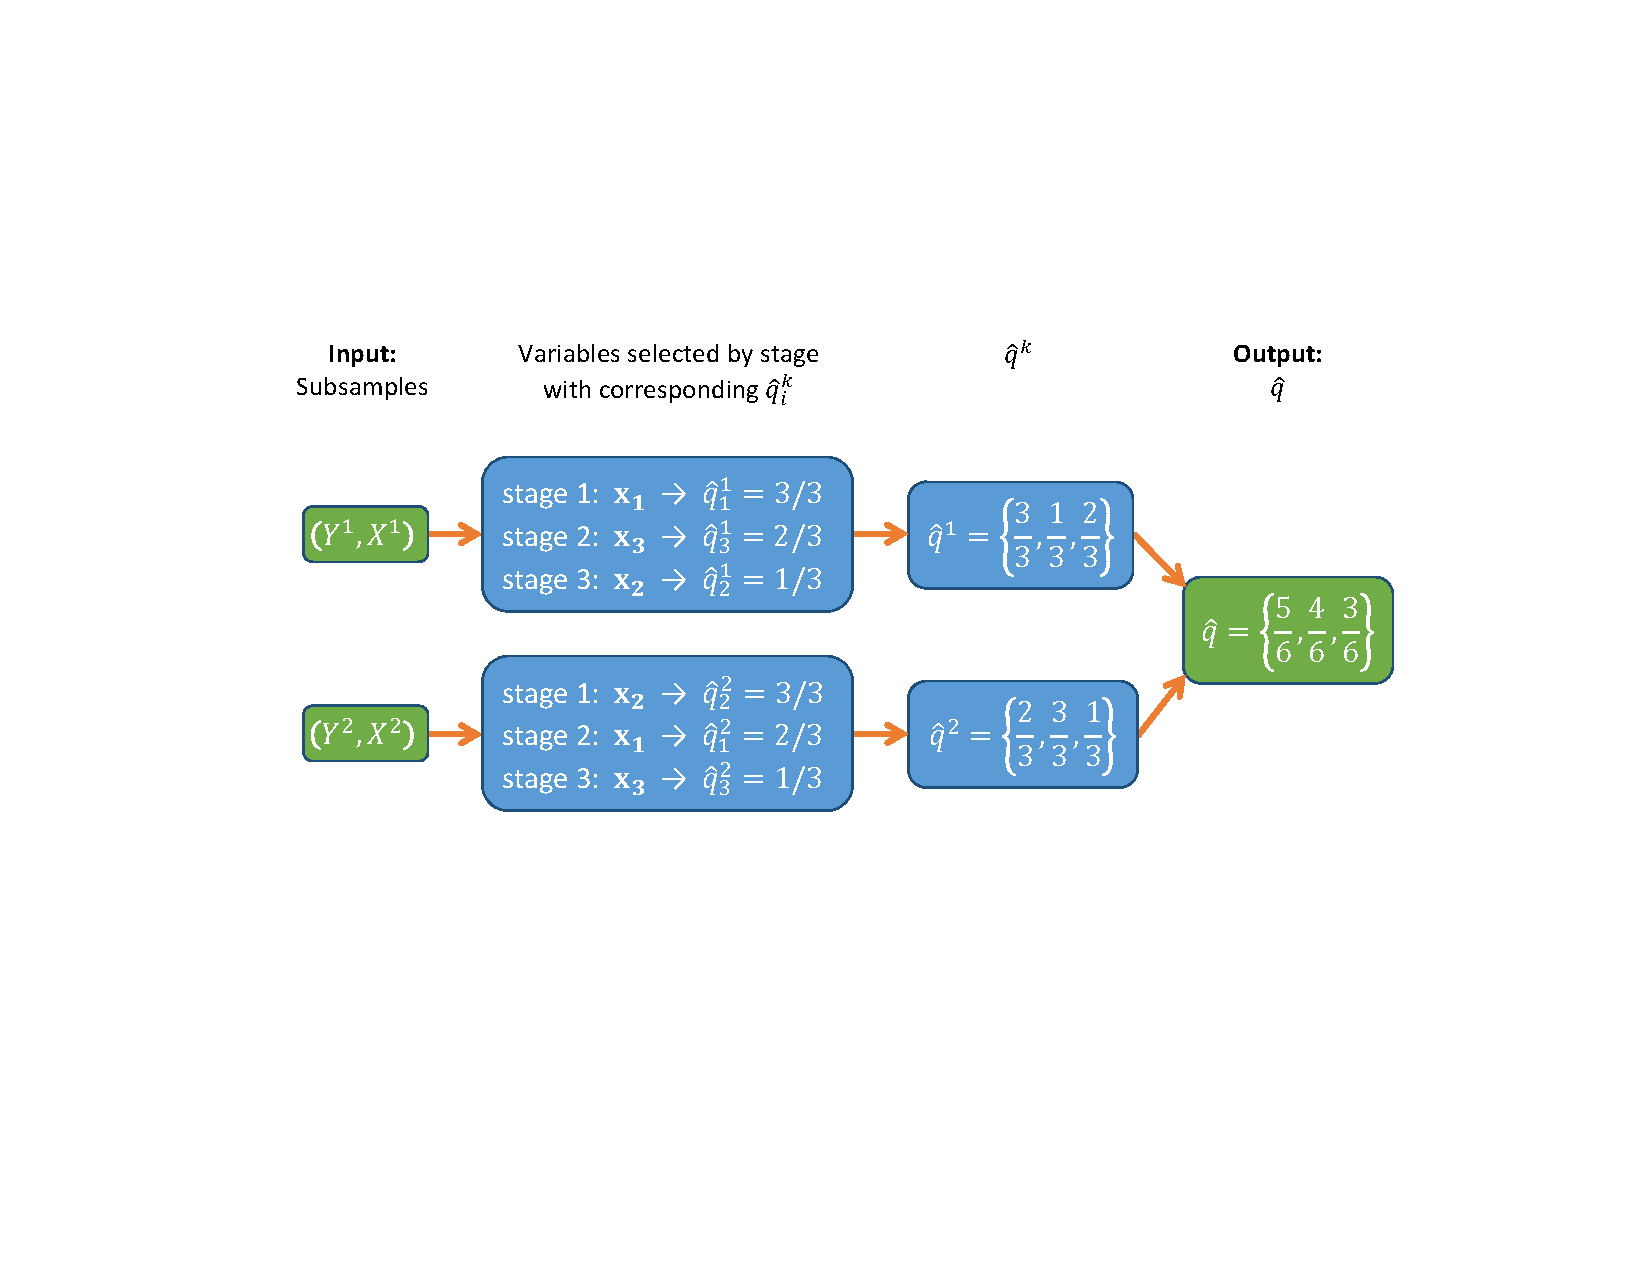
\includegraphics[width=0.66\paperwidth]{q_demo_1new.pdf}
%
  \caption{Computation of $\widehat{q}$ on 2 subsamples where $\left\{ \mathbf{x}_1, \mathbf{x}_2 \right\}$ are informative and $\mathbf{x}_3$ redundant.}
%
  \label{fig:q_demo}
%
\end{figure}

The first step in Algorithm~\ref{algo:APE-lar}, without loss of generality, generates subsamples without replacement. The second step (lines~\ref{inner_averaging_start}-\ref{inner_averaging_end}) computes $\widehat{q}^k$, which summarizes the order that least angle regression includes each $\mathbf{x}_i$ across all stages (as in the Figure~\ref{fig:q_demo} example). The unrestricted least-angle regression only ranks variables by the stage $\mathbf{x}_i$ enters the solution path. As shown in line~\ref{inner_averaging_end} of Algorithm~\ref{algo:APE-lar} and Figure~\ref{fig:q_demo}, variables included at earlier stages have larger corresponding $\widehat{q}^k_i$ values: the first variable included is assigned $1$, the last is assigned $1/\widetilde{p}$ and the dropped variables are assigned $0$ (which occurs only when $p > n$). Thus, by ranking (decreasingly) the $\mathbf{x}_i$ according to their corresponding $\widehat{q}^k_i$ values, we obtain the $L_0$ solution path. The \citet[Theorem 2]{zhang09} result implies that the variables with the largest $\widehat{q}^k_i$ values, on average, are more likely to be informative variables. The $\widehat{q}^k_i$ may be sensitive in high-dimensional spaces to multicollinearity, sampling randomness and noise. A consequence is that a redundant variable may be included at an early stage in some subsample $\left( Y^k, X^k \right)$. Consider Figure~\ref{fig:q_demo}, where $\mathbf{x}_1$ and $\mathbf{x}_2$ are informative and $\mathbf{x}_3$ is redundant. In subsample $\left( Y^1, X^1 \right)$ at stage 2, the redundant variable $\mathbf{x}_3$ is included, implying $\widehat{q}^1_3$ (the $\widehat{q}^k_i$ value for $\mathbf{x}_3$ in $\left( Y^1, X^1 \right)$) is larger than $\widehat{q}^1_2$ (the $\widehat{q}^k_i$ value for the informative variable $\mathbf{x}_2$ in $\left( Y^1, X^1 \right)$). The third step in Algorithm~\ref{algo:APE-lar} (lines~\ref{outer_averaging_start}-\ref{outer_averaging_end}) reduces the impact of sensitivity in the $\widehat{q}^k_i$ values by computing $\widehat{q} := \frac{1}{K} \sum_{k=1}^{K} \widehat{q}^k$ and ranking the $\mathbf{x}_i$ (decreasingly) based on the corresponding value of $\widehat{q}_i$ (the $i$\textsuperscript{th} entry of $\widehat{q}$), to get the average $L_0$ solution path. The average $L_0$ solution path is formally defined as follows.
%
\begin{definition}[average $L_0$ solution path]
  %
  Define the \textbf{average $L_0$ solution path} of forward regression on $\left\{ \left( Y^k, X^k \right) \right\}_{k=1}^{K}$ to be the decreasing rank order of variables based on their corresponding $\widehat{q}_i$ values. For example, in Figure~\ref{fig:q_demo}, the $\widehat{q}_i$ values for $\mathbf{x}_1$, $\mathbf{x}_2$ and $\mathbf{x}_3$ are, respectively, $\widehat{q}_1 = 5/6$, $\widehat{q}_2 = 4/6$ and $\widehat{q}_3 = 3/6$. As a result, the average $L_0$ solution path can be represented as an ordered set $\left\{ \left\{ \mathbf{x}_1 \right\}, \left\{ \mathbf{x}_1, \mathbf{x}_2 \right\}, \left\{ \mathbf{x}_1, \mathbf{x}_2, \mathbf{x}_3 \right\} \right\}$.
  %
  \label{def:L_0_solution_path}
  %
\end{definition}

%%%%%%%%%%%%%%%%%%%%%%%%%%%%%


\begin{algorithm}[h]

  \SetKwData{Left}{left}\SetKwData{This}{this}\SetKwData{Up}{up}
  \SetKwFunction{Union}{Union}\SetKwFunction{FindCompress}{FindCompress}
  \SetKwInOut{Input}{input}\SetKwInOut{Output}{output}

  \smallskip
  Randomly select 20\% of the sample points as the validation set; denote the remaining points as the training set\;

  Estimate $\widehat{q}$ using Algorithm~\ref{algo:APE-lar} on the training set and compute $Q(c) = \left\{ \mathbf{x}_j \; \vert \; \widehat{q}_j \geqslant c, \forall j\right\}$ for all $c \in \left\{ 1, 0.98, \ldots, 0.02, 0 \right\}.$

  Run an OLS regression of each $Q(c)$ to $Y$ on the training set and find $c^*$, the value of $c$ that minimizes the validation error\;

  Compute the OLS coefficients of $Q(c^*)$ to $Y$ on the whole sample.

  \caption{Subsample-ordered least-angle regression \label{algo:solar}}
\end{algorithm}

Built on Algorithm~\ref{algo:APE-lar}, the solar algorithm is summarized in Algorithm~\ref{algo:solar}. Instead of the equiangular, partial-correlation search in least-angle regression, variables are included into forward regression according to their rank order in the average $L_0$ solution path, represented by $\left\{ Q(c) \vert c = 1, 0.98, \ldots, 0\right\}$ in Algorithm~\ref{algo:solar}. We use $\widehat{q}$ from Algorithm~\ref{algo:APE-lar} to generate a list of variables $Q \left( c \right) = \left\{ \mathbf{x}_j \; \vert \; \widehat{q}_j \geqslant c, \forall j \leqslant p \right\}$. For any $c_1 > c_2$, $Q\left(c_1\right) \subset Q\left(c_2\right)$, implying a sequence of nested sets $\left\{ Q(c) \vert c = 1, 0.98, \ldots, 0\right\}$. Each $c$ denotes a stage of forward or least-angle regression. For a given value of $c$, $Q(c)$ denotes the set of variables with $\left\Vert \beta_i \right\Vert_0=1$ on average and $Q(c) - Q(c - 0.02)$ is the set of variables with $\left\Vert \beta_i \right\Vert_0$ just turning to $1$ at $c$. Therefore, $\left\{ Q(c) \vert c = 1, 0.98, \ldots, 0\right\}$ is the average $L_0$ solution path of Definition~\ref{def:L_0_solution_path}. Variables that are more likely to be informative are included at $Q(c)$ with larger value of $c$, which will be selected first by the solar algorithm. Note that Algorithm~\ref{algo:solar} can be easily adapted to different requirements. For example, we can replace the forward regression setting in Algorithm~\ref{algo:solar} with least-angle regression if shrinkage is preferred in variable selection (for example, in Reproducing kernel Hilbert spaces). Moreover, backwards elimination, proposed by \citet{zhang09} for sparsity improvement, can be added at the end of Algorithm~\ref{algo:solar}.


\subsection{Solar solved by coordinate descent}

The solar algorithm can be easily generalized to coordinate descent scheme. Both least-angle regression and coordinate descent generate a solution path for lasso, parametrized with $\beta_i$ on vertical axis and tuning parameter $t$ or $\lambda$ on horizontal axis. Hence, to reprogram solar using coordinate descent, we just need to replace Algorithm~\ref{algo:APE-lar} with Algorithm~\ref{algo:APE-cd}, which records the order of variable activation along the coordinate descent solution path.

\smallskip
\begin{algorithm}[h]

  \SetKwData{Left}{left}\SetKwData{This}{this}\SetKwData{Up}{up}
  \SetKwFunction{Union}{Union}\SetKwFunction{FindCompress}{FindCompress}
  \SetKwInOut{Input}{input}\SetKwInOut{Output}{output}

  \smallskip
  \Input{$\left( Y, X \right)$.}

  generate $K$ subsamples $\left\{ \left( Y^k, X^k \right) \right\}^{K}_{k=1}$ by randomly remove $1/K$ of observations in $\left( Y, X \right)$\;

  set $\widetilde{p} = \min\left\{ n_{\mathrm{sub}}, p \right\}$ \;

  \For{ k := 1 to K, stepsize = 1 \nllabel{outer_averaging_start} }{

    denote $\lambda_s$ as the $\lambda$ value that coordinate descent lasso includes $s$ variables, $\forall s \in \left(0, \widetilde{p}\right]$; 

    run a coordinate descent lasso on $\left( Y^k, X^k \right)$, $\forall \lambda \in \left\{\lambda_1, \ldots, \lambda_{\widetilde{p}},\right\}$
    
    record the order of variable inclusion at each $\lambda \in \left\{ \lambda_1, \ldots, \lambda_{\widetilde{p}},\right\}$\;

    define $\widehat{q}^k = \mathbf{0} \in \mathbb{R}^p$\;

    for all $i$ and $s$, if $\mathbf{x}_i$ is included at $\lambda = \lambda_s$, set $\widehat{q}^k_i= (\widetilde{p} + 1 - s) / \widetilde{p}$, where $\widehat{q}^k_i$ is the $i$\textsuperscript{th} entry of $\widehat{q}^k$\;

  }

  $\widehat{q} := \frac{1}{K} \sum_{k=1}^{K} \widehat{q}^k$\; \nllabel{outer_averaging_end}

  \Return $\widehat{q}$

\caption{average $L_0$ path estimation via coordinate descent \label{algo:APE-cd}}

\end{algorithm}

\begin{figure}[h]
  %
  \centering
  %
  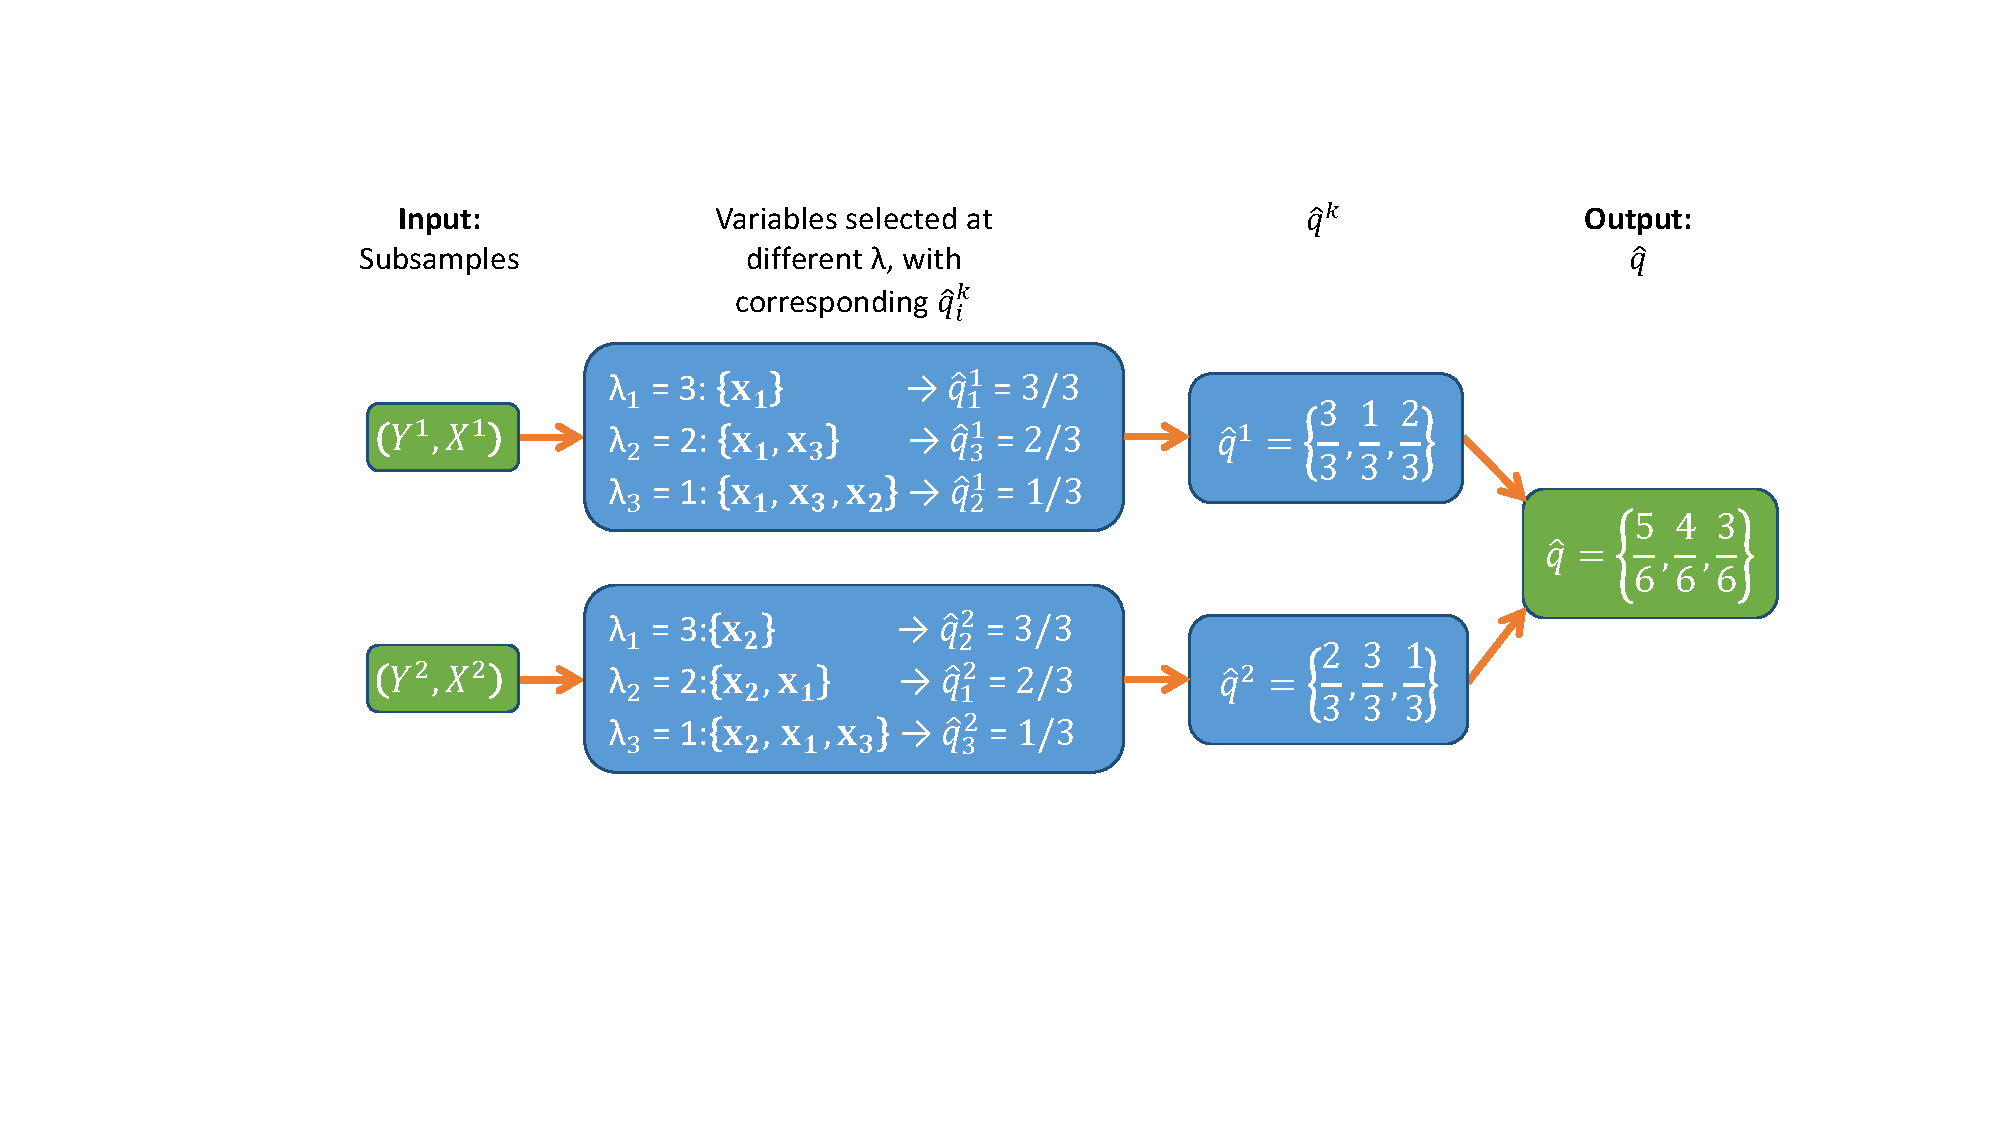
\includegraphics[width=0.66\paperwidth]{q_demo_3.pdf}
  %
  \caption{Computation of $\widehat{q}$ on 2 subsamples using coordinate descent.}
  %
  \label{fig:q_demo_3}
  %
\end{figure}

Algorithm~\ref{algo:APE-cd} estimates the average $L_0$ path via coordinate descnet, serving the same purpose as Algorithm~\ref{algo:APE-lar}. Compared to Algorithm~\ref{algo:APE-lar}, Algorithm~\ref{algo:APE-cd} use $\lambda$ to record the order that each variale enters the path. Let's take Figure~\ref{fig:q_demo_3} as an example. To parametrize the solution path, we denote $\lambda_s$ as the $\lambda$ value that coordinate descent lasso includes $s$ variables, $\forall s\in \left( 0, \min \left\{ n/2, p \right\} \right]$. Hence, we define a sequence of $\lambda$ for grid search. In each subsample $\left( Y^k, X^k \right)$, we train a standard coordinate descent lasso, allowing $\lambda$ value to stepwise increase within the grid $\left\{\lambda_1, \ldots, \lambda_{ \min \left\{ n/2, p \right\} } \right\}$, where $\lambda_1 \geqslant \ldots \geqslant \lambda_{ \min \left\{ n/2, p \right\} }$. In Figure~\ref{fig:q_demo_3}, when $\lambda < \lambda_3$ at subsample $\left( Y^1, X^1 \right)$, all three variables are activated in the solution path, implying that $\widehat{q}^1_i \geqslant 1/3$ for all variables. When $\lambda$ value increases to $\lambda_2$, only $\{\mathbf{x}_3, \mathbf{x}_1\}$ survive the harsher shrinkage, implying that they should be ranked higher than $\mathbf{x}_2$. As a result, $\widehat{q}^1_1, \widehat{q}^1_3 \geqslant 2/3$ and $\widehat{q}^1_2 = 1/3$. When $\lambda$ value hits $\lambda_3$, only $\{\mathbf{x}_1\}$ remains activated, leaving $\widehat{q}^1_1 = 3/3$ and $\widehat{q}^1_3 = 2/3$. Afterwards, we can apply the same calculation method to each subsample, resulting in the same $\widehat{q}$ as Algorithm~\ref{algo:APE-lar} does. 

The coordinate descent generalization has several influences. Firstly, many lasso-type estimators rely on coordinate descent; hence, the solar-cd generalization implies that solar can be applied to all lasso-type problems. Secondly, although \cite{tibshirani2015general} shows explicitly that the computational efficiency and accuracy of least-angle regression are quite on par with coordinate descent in a number of applications, coordinate descent is still considerd the most computationallly efficient in gerenal applications; as a result, the coordinate descent generalization improves the computational performance in a number of scenarios. Both solar and its coordinate descent generalization can be easily programmed using any lasso packages, such as GPU-based version \citep{fujiwara2016fast} and Python-interfaced Fortran/C++ version \citep{scikit-learn}. In this paper, we stick to the \citet{scikit-learn} source code and program everything using Python-interfaced Fortran/C++ for the maximum performance, assuming without a NVidia GPU.


\section{Solar improvements over forward regression, lasso rules and traditional variable screening \label{section:adv}}

Solar has several clear advantages. Firstly, it solves Example~1 type problems. Because solar relies on a single, average $L_0$ solution path and a fixed training-validation split to determine $c^*$, each value of $c$ is mapped to a unique set of selected variables. Secondly, solar is amenable to post-selection testing. In particular, because covariance tests \citep{lockhartall14} and spacing tests \citep{taylor2014exact}) are based on forward or least-angle regression, they are potentially adaptable to solar. Moreover, we can easily modify the data-splitting tests \citep{wasserman2009high,meinshausen2009p} with many classical test staistics. We illustrate this point using Example~3.

\bigskip
\noindent
\textbf{Example 3.} Suppose $Y = 2 \mathbf{x}_0 + 3 \mathbf{x}_1 + 4 \mathbf{x}_2 + 5 \mathbf{x}_3 + 6 \mathbf{x}_4  + e$, where all $\mathbf{x}_i$ and $e$ are standard Gaussian with pairwise correlations of $0.5$. Post-selection tests are typically applied with sufficiently large $n$, so $p/n=50/100$. In this setting, forward regression (FR) selects $\left[\mathbf{x}_4, \mathbf{x}_3, \mathbf{x}_2, \mathbf{x}_1, \mathbf{x}_0, \mathbf{x}_{45}, \mathbf{x}_{8}, \mathbf{x}_{40}, \mathbf{x}_{6}, \mathbf{x}_{39}, \mathbf{x}_{11}, \mathbf{x}_{34}, \mathbf{x}_{5} \right]$ using BIC score minimization. By contrast, solar selects only $\left[\mathbf{x}_4, \mathbf{x}_3, \mathbf{x}_2, \mathbf{x}_1, \mathbf{x}_0, \mathbf{x}_{45}, \mathbf{x}_{40} \right]$. We then conduct post-FR and post-solar t-tests and compare the results to the OLS regression of $Y$ on the $\mathbf{x}_i$.

After standardizing the $\mathbf{x}_i$ and $\mathbf{Y}$, the sample regression coefficient is identical to the corresponding conditional correlation. Both the t-test results and FR selection decisions are largely based on the sample regression coefficient absolute values; keeping variables with large values and purging the rest. Hence, the variables selected by FR also have low p-values on the current sample, implying that direct, post-FR t-tests overfit the sampling randomness that also affects the variable selection algorithm (referred to as `p-value overfitting'). The key issue here is that there is no sample change between the FR sample and the post-FR test sample.

To solve this issue, we improve the data-splitting teststhe with \citet{bousquet2002stability} method --- a Jackknife-type algorithm --- as follows: after solar selection on the whole sample, we randomly divide the sample into $K$ folds, remove each fold in turn, and compute the t-values of post-solar OLS on the remaining $K-1$ folds. We calculate the average t valuess and se in $K$ rounds and call the $K=2$ version the \emph{hold-out average}. The traditional \citet{wasserman2009high, meinshausen2009p} methods only use a fraction of the sample for selection and testing; by contrast, our method guarantees the whole sample for selection and applies a Jackknife-type algorithm for the maximum sample utilization on testing.

As shown in Table~\ref{table:post-selection-test}, the hold-out average t-values for $\left[\mathbf{x}_4, \mathbf{x}_3, \mathbf{x}_2, \mathbf{x}_1, \mathbf{x}_0\right]$ are very similar to their OLS counterparts while the hold-out average t-values for $\left[\mathbf{x}_{40}, \mathbf{x}_{45} \right]$ are lower, which leads to purging $\mathbf{x}_{40}$ and $\mathbf{x}_{45}$. We repeat the simulation 200 times and the results, summarized in Figure~\ref{fig:t_value_compare}, confirm that improvements in the hold-out average are not simply due to chance. It is important to note that OLS uses all of the sample and has $50$ residual degrees of freedom whereas the hold-out average uses only 50\% of the sample in each round and consequently has $30$-$40$ degrees of freedom. Thus, the hold-out average naturally produces slightly lower t-values for $\left[\mathbf{x}_4, \mathbf{x}_3, \mathbf{x}_2, \mathbf{x}_1, \mathbf{x}_0\right]$ and the t-value boxplots for the hold-out average are slightly less concentrated than the OLS boxplots. Simulations in Section~\ref{subsection:suml1}, show that solar supplemented with the hold-out average purges almost all of the redundant variable while retaining all of the informative variables.

%\smallskip
\begin{table}[h]
\centering
\caption{Comparison of post-selection t tests between FR, hold-out average, and OLS.}
\label{table:post-selection-test}
\renewcommand{\arraystretch}{0.7}
  \begin{tabular}{l............}
    \toprule
    & \multicolumn{3}{c}{post-FR} & \multicolumn{3}{c}{hold-out average} & \multicolumn{3}{c}{classical OLS} \\
    \cmidrule(lr){2-4} \cmidrule(lr){5-7} \cmidrule(lr){8-10}
    & \multicolumn{1}{c}{$se$} & \multicolumn{1}{c}{$t$} & \multicolumn{1}{c}{$P>\left\vert t \right\vert$ } & \multicolumn{1}{c}{$se$} & \multicolumn{1}{c}{$t$} & \multicolumn{1}{c}{$P>\left\vert t \right\vert$} & \multicolumn{1}{c}{$se$} & \multicolumn{1}{c}{$t$} & \multicolumn{1}{c}{$P>\left\vert t \right\vert$} \\
    \cmidrule{1-10}
    $\mathbf{x}_0$ & 0.12 & 15.68 & 0 & 0.18 & 11.34 & 0 & 0.19 & 9.85 & 0 \\
    $\mathbf{x}_1$ & 0.14 & 20.06 & 0 & 0.22 & 12.76 & 0 & 0.23 & 12.05 & 0 \\
    $\mathbf{x}_2$ & 0.14 & 28.11 & 0 & 0.21 & 18.22 & 0 & 0.20 & 19.45 & 0 \\
    $\mathbf{x}_3$ & 0.13 & 39.19 & 0 & 0.20 & 24.48 & 0 & 0.20 & 25.08 & 0 \\
    $\mathbf{x}_4$ & 0.13 & 42.34 & 0 & 0.21 & 27.36 & 0 & 0.20 & 28.15 & 0 \\
    $\mathbf{x}_{40}$ & 0.12 & 2.59 & 0.01 & 0.19 & 1.90 & 0.18 & 0.18 & 2.36 & 0.02 \\
    $\mathbf{x}_{45}$ & 0.13 & 2.30 & 0.02 & 0.21 & 1.19 & 0.25 & 0.19 & 1.60 & 0.12 \\
    \bottomrule
  \end{tabular}
\end{table}
\smallskip


\begin{figure}[h]
%
  \centering
%
  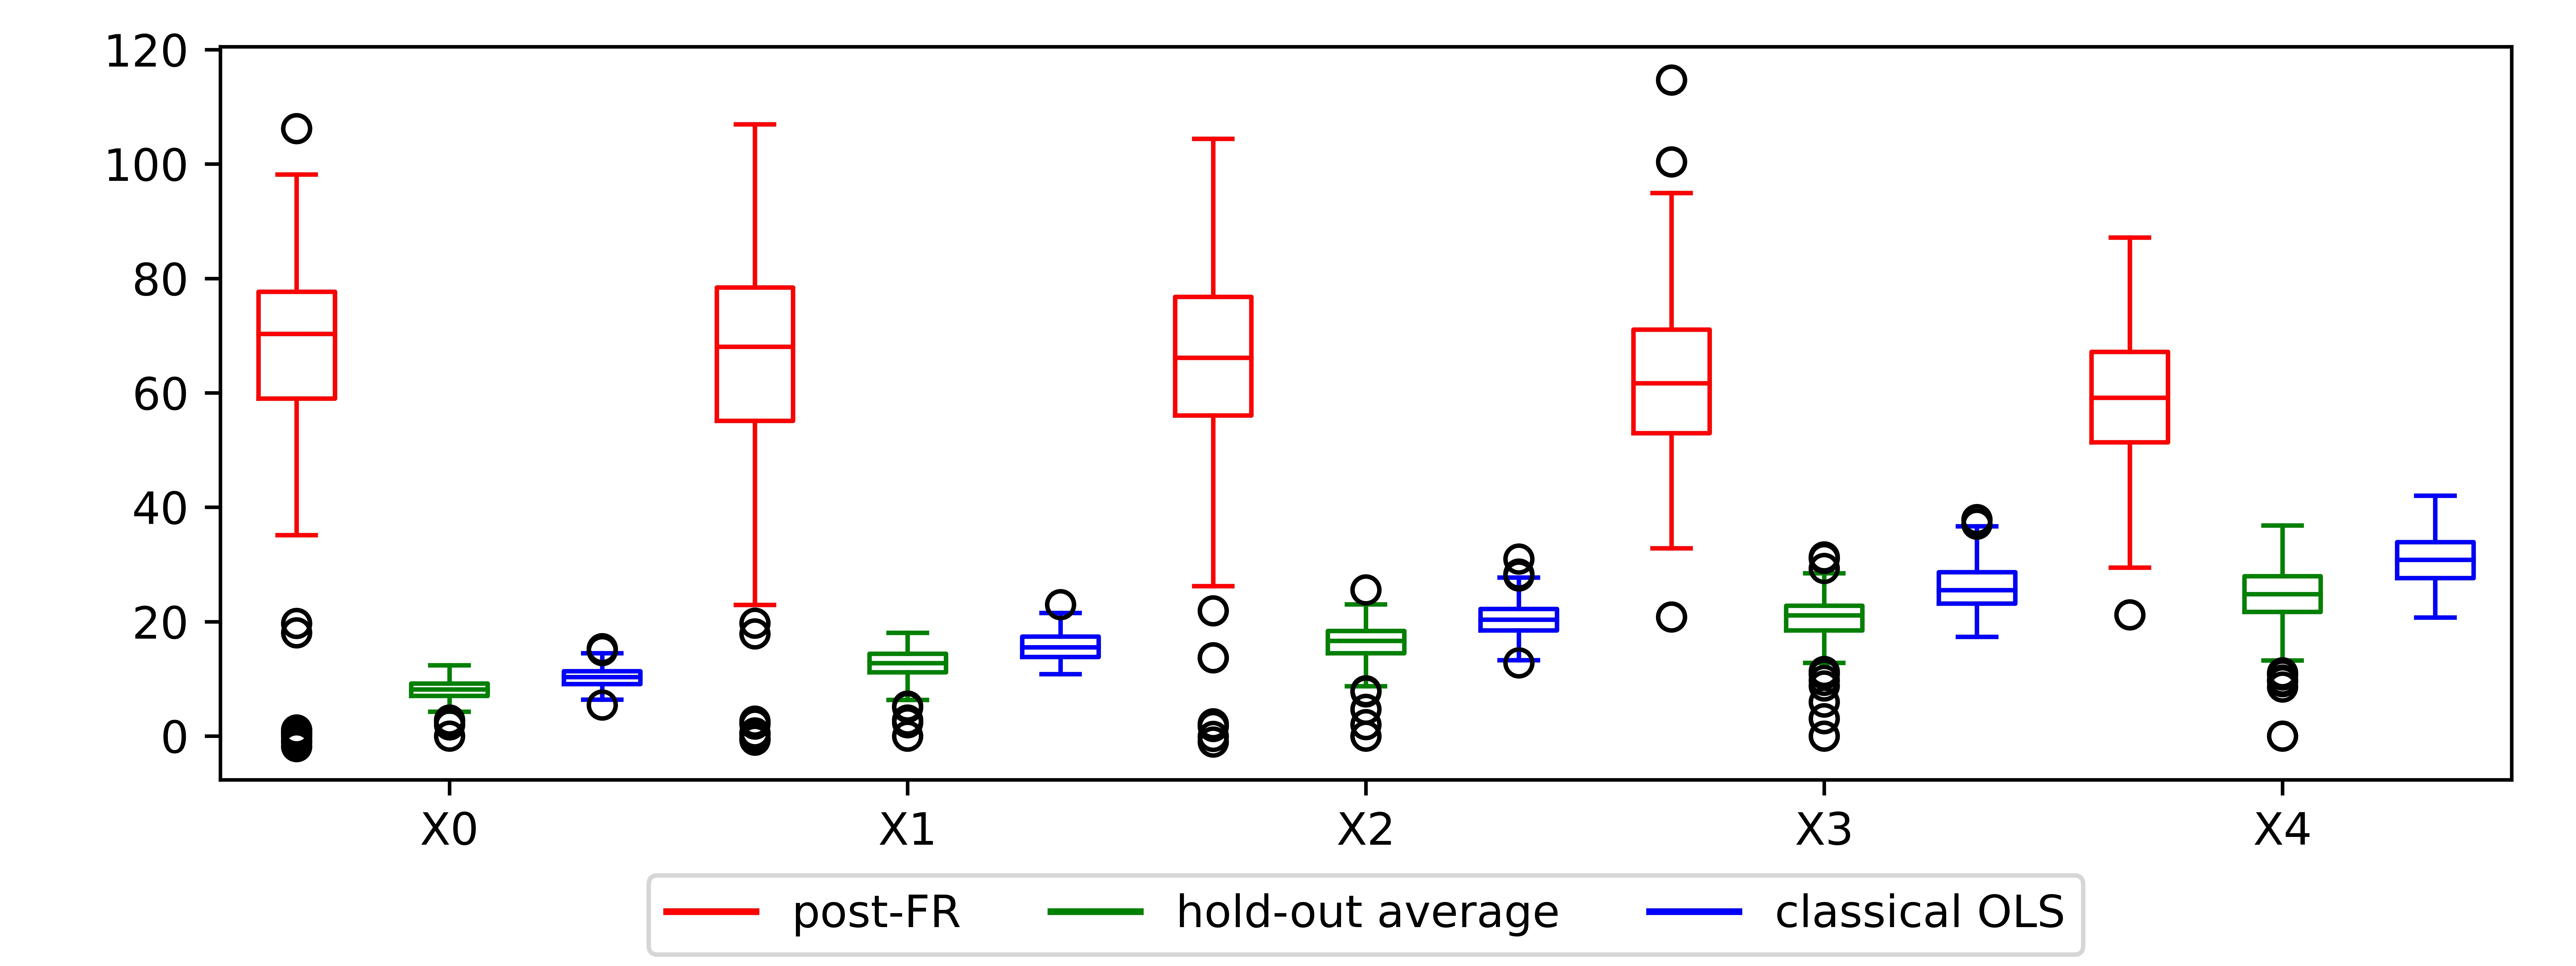
\includegraphics[width=0.7\paperwidth]{t_value_compare.jpg}
%
  \caption{Boxplots of post-selection t values from FR, hold-out average, and OLS.}
%
  \label{fig:t_value_compare}
%
\end{figure}

While the hold-out average procedure can be applied to other methods, solar has several intrinsic advantages. Firstly, to ensure accurate tests with only half the sample, it is important to retain residual degrees of freedom, implying that variable selection must be as sparse and accurate as possible. As shown in section~\ref{section:comp} and \ref{section:application}, sparse and accurate selection is one of the benefits of solar. Secondly, compared to FR and lasso, the average $L_0$ path of solar is robust to settings of the irrepresentable condition, sampling noise, multicollinearity and other issues, which benefits post-selection tests when deciding which $\beta_i$ to test. A larger $K$ is needed in smaller samples for a larger residual degree of freedom. To conclude, this example illustrates the possibility that the hold-out average may significantly reduce the severity of `p-value overfitting' while utilizing as many data points as possible for selection and testing. This method helps reduce the severity of informative variable omission or redundant variable inclusion. $\blacksquare$

\subsection*{Solar selection advantages under complicated dependence structure}

Indeed, solar has another advantage: the average $L_0$ solution path offers additional robustness against subsampling randomness, multicollinearity, noise and outliers in high-dimensional spaces. Thus, solar is likely to be more reliable than other variable selection methods under complicated dependence structures. We illustrate the point with the following two Bayesian network examples.

\begin{figure}[h]
%
  \centering
  %
  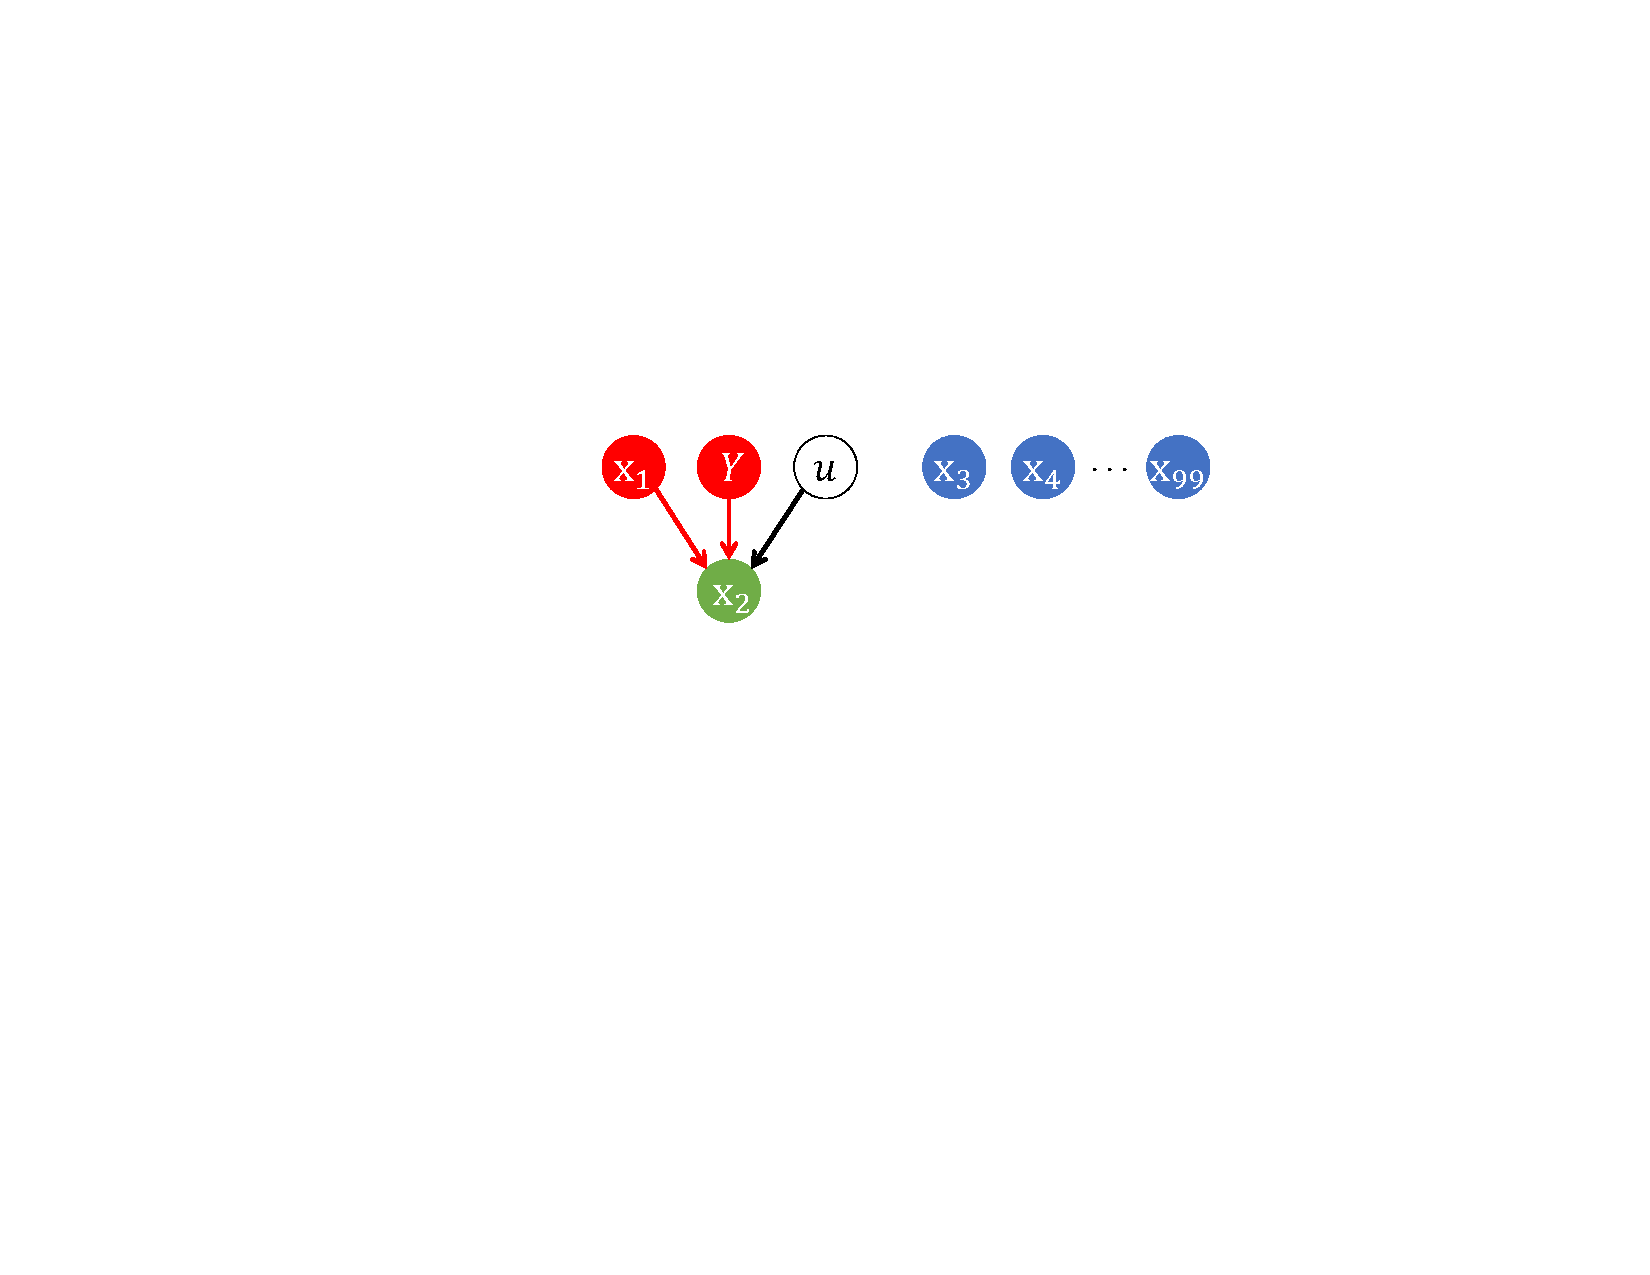
\includegraphics[width=0.35\paperwidth]{uncond_example.pdf}
  %
  \caption{Collider structure for $\mathbf{x}_2$ with latent $u$.}
  %
  \label{fig:uncond_example}
%
\end{figure}

Consider the non-standard regression case in Figure~\ref{fig:uncond_example}, where $Y$ has two informative variables: a spouse ($\mathbf{x}_1$) and a child ($\mathbf{x}_2$). Figure~\ref{fig:uncond_example} depicts a common scenario in empirical regression: \emph{informative variables} may be \emph{unconditionally uncorrelated to} $Y$ in the DGP. With such data, Example~4 demonstrates that forward regression (including solar and lasso) is more reliable than post-lasso rules and variable screening.

\smallskip
\noindent
\textbf{Example 4.} In Figure~\ref{fig:uncond_example}, there are $100$ variables and $\mathbf{x}_2$ is (causally) generated by its parents $\left\{ \mathbf{x}_1, Y \right\}$ as follows,
%
\begin{equation}
  %
  \mathbf{x}_2 = \alpha_1 \mathbf{x}_1 + \alpha_2 Y + u,
  %
  \label{eqn:collider_1}
  %
\end{equation}
%
where $\mathbf{x}_1$ is unconditionally uncorrelated with $Y$, $\mathbf{x}_1$ and $Y$ are both unconditionally and conditionally uncorrelated with any redundant variable, $\left\{\alpha_1, \alpha_2 \right\}$ are population regression coefficients and $u$ is a Gaussian noise term. If $Y$ is chosen to be the response variable, we have the population regression equation
%
\begin{equation}
  %
  Y = -\frac{\alpha_1}{\alpha_2} \mathbf{x}_1 + \frac{1}{\alpha_2} \mathbf{x}_2 - \frac{1}{\alpha_2}u.
  %
  \label{eqn:collider_2}
  %
\end{equation}
%
Note that $\mathbf{x}_1$ and $\mathbf{x}_2$ are both informative variables for $Y$. However, since $\mathbf{x}_1$ is unconditionally uncorrelated with $Y$ in the population, some post-lasso rules (such as the strong rule \citep{tibshirani2012strong} and the safe rule \citep{ghaoui2010safe}) may be prone to purging $\mathbf{x}_1$ incorrectly. Given the value of shrinkage parameter $\lambda$ in a grid search, the base strong rule and the safe rule for lasso purge any selected variable that satisfies, respectively, (\ref{eqn:safe_rule}) and (\ref{eqn:strong_rule}):
%
\begin{eqnarray}
  %
  \left\vert \mathbf{x}_i^T Y \right\vert < & \lambda - \left\Vert \mathbf{x}_i \right\Vert_2 \left\Vert Y \right\Vert_2 \frac{\lambda_{max} - \lambda} {\lambda_{max}} ; \label{eqn:safe_rule} \\
  %
  \left\vert \mathbf{x}_i^T Y \right\vert < & 2\lambda - \lambda_{max} , \label{eqn:strong_rule}
  %
  \label{eqn:post_estmation_rule}
  %
\end{eqnarray}
%
where the $\mathbf{x}_i$ are standardized and $\lambda_{max}$ is the value of $\lambda$ that purges all the variables. Both rules are based on the unconditional covariance between $\mathbf{x}_i$ and $Y$. For a given value of $\lambda$ (typically selected by CV), lasso likely will select $\mathbf{x}_1$ and $\mathbf{x}_2$ along with some redundant variables from $\left\{ \mathbf{x}_3, \ldots, \mathbf{x}_{99} \right\}$ (since the DGP does not violate any IRC). Since $\mathrm{corr} \left( \mathbf{x}_1, Y \right) = \mathrm{corr} \left( \mathbf{x}_3, Y \right) =  \cdots = \mathrm{corr} \left( \mathbf{x}_{99}, Y \right) = 0$ in the population, the sample value of $\left\vert \mathbf{x}_1^T Y \right\vert$ will be approximately as small as the $\left\vert \mathbf{x}_i^T Y \right\vert$ of any redundant variable. Put another way, $\mathbf{x}_1$ cannot be distinguished from the redundant variables by the value of $\left\vert \mathbf{x}_i^T Y \right\vert$. To ensure $\mathbf{x}_1$ is not purged by (\ref{eqn:safe_rule}) or (\ref{eqn:strong_rule}), both $\lambda - \left\Vert \mathbf{x}_1 \right\Vert_2 \left\Vert Y \right\Vert_2 \frac{\lambda_{max} - \lambda} {\lambda_{max}}$ and $2\lambda - \lambda_{max}$ must be smaller than $\left\vert \mathbf{x}_1^T Y \right\vert$. However, this will lead to two problems. First, decreasing the right-hand side of (\ref{eqn:safe_rule}) and (\ref{eqn:strong_rule}) will reduce the value of $\lambda$, implying that lasso will select more redundant variables. Second, since $\left\vert \mathbf{x}_1^T Y \right\vert$ will be approximately as small as the $\left\vert \mathbf{x}_i^T Y \right\vert$ of any redundant variable selected by lasso, not purging $\mathbf{x}_1$ (by reducing both right-hand side terms) may result in (\ref{eqn:safe_rule}) and (\ref{eqn:strong_rule}) retaining redundant variables.

Variable screening methods \citep{fan2008sure} may also be prone to selecting redundant variables. Screening ranks variables decreasingly based on the absolute values of their unconditional correlations to $Y$, selecting the top $w$ variables (with $w$ selected by CV, bootstrap or BIC). Since $\mathrm{corr} \left( \mathbf{x}_2, Y \right) \neq 0$ in the population, screening will rank $\mathbf{x}_2$ highly. However, it may not rank $\mathbf{x}_1$ highly because $\mathrm{corr} \left( \mathbf{x}_1, Y \right) = 0$ in the population. Thus, some redundant variables may be ranked between $\mathbf{x}_2$ and $\mathbf{x}_1$, implying that if both $\mathbf{x}_1$ and $\mathbf{x}_2$ are selected, screening will select redundant variables.

The average $L_0$ solution path will not suffer the same problem. For convenience, assume $-\alpha_1 / \alpha_2 > 0$ and $p/n = 100/200$ or smaller. For lars, as we increase $\left\Vert \beta_2 \right\Vert_1$ at stage~1 (i.e., as we `partial' $\mathbf{x}_2$ out of $Y$), the unconditional correlation between $Y - \beta_2 \mathbf{x}_2$ and $\mathbf{x}_1$ will increase above $0$ significantly while the marginal correlation between $Y - \beta_2 \mathbf{x}_2$ and any redundant variable will remain approximately $0$. Thus, in the $L_0$ solution path and, hence, the average $L_0$ solution path, $\mathbf{x}_1$ will be included immediately after $\mathbf{x}_2$ is included. $\blacksquare$

\bigskip
In the second example, we revisit Example~2, which illustrates another common scenario in empirical regression: \emph{redundant variables} may be \emph{unconditionally correlated to} $Y$ in the DGP. In this example, we choose specific values for $\beta_1$, $\beta_2$, $\omega$ and $\delta$ to demonstrate that, even when IRC is satisfied, the strong rule, base rule and variable screening methods may have difficulty purging the redundant $\mathbf{x}_3$. By contrast, solar is more reliable.

\bigskip
\noindent
\textbf{Example 2 revisited.} Consider the following confounding structure,
%
\begin{equation}
	%
	\begin{cases}
	%
    \mathbf{x}_3 = \frac{1}{3} \mathbf{x}_1 + \frac{1}{3} \mathbf{x}_2 + \frac{\sqrt{7}}{3} u, \\
    %
    Y = \frac{7}{10} \mathbf{x}_1 +  \frac{2}{10} \mathbf{x}_2 +  \frac{\sqrt{47}}{10} e. \\
    %
	\end{cases}
	%
	\label{eqn:example_4}
	%
\end{equation}
%
where $\mathbf{x}_1$ and $\mathbf{x}_2$ cause both $Y$ and $\mathbf{x}_3$, implying that $\mathbf{x}_3$ is unconditionally correlated to $Y$; $\mathbf{x}_1$, $\mathbf{x}_2$, $u$ and $e$ are independent; $\mathbf{x}_3$ is independent from $e$; $Y$ is independent from $u$; and all variables are standardized. When $n$ is large and the sample correlations close to their population values, the sample marginal correlations to $Y$ can be ranked in decreasing order,
%
\begin{equation}
  %
  \begin{aligned}
    %
    \mathrm{corr} \left( \mathbf{x}_1, Y \right)  = & \;0.7 \\
    %
    \mathrm{corr} \left( \mathbf{x}_3, Y \right)  = & \;\mathrm{corr} \left( \frac{1}{3} \mathbf{x}_1 + \frac{1}{3} \mathbf{x}_2, \frac{7}{10} \mathbf{x}_1 +  \frac{2}{10} \mathbf{x}_2 \right)
    %
    = 0.3. \\
    %
    \mathrm{corr} \left( \mathbf{x}_2, Y \right)  = & \;0.2 \\
    %
  \end{aligned}
  %
\end{equation}
%
Because $\mathbf{x}_2$ ranks below $\mathbf{x}_1$ and $\mathbf{x}_3$ in terms of marginal correlations to $Y$, the variable screening method will have to select all $3$ variables, including the redundant $\mathbf{x}_3$, to avoid omitting $\mathbf{x}_2$. Similarly, the base strong rule and safe rule may also have difficulty purging $\mathbf{x}_3$. Because $\mathrm{corr} \left( \mathbf{x}_3, Y \right)$ is larger than $\mathrm{corr} \left( \mathbf{x}_2, Y \right)$, if lasso selects both $\mathbf{x}_3$ and $\mathbf{x}_2$ and we use the base strong rule or the safe rule to purge $\mathbf{x}_3$, we will also have to purge $\mathbf{x}_2$.

Forward regression and lars will not make the same errors. Because (\ref{eqn:example_4}) does not violate the IRC, variable-selection consistency of forward regression and lars is assured by the theoretical results of \citet{zhang09} and \citet{zhaoyu06}. Specifically in forward regression, $\mathbf{x}_1$ will be included  at the first stage. After controlling for $\mathbf{x}_1$, the partial correlations to $Y$ of both $\mathbf{x}_2$ and $\mathbf{x}_3$ can be ranked in decreasing order as follows (when $n$ is large),
%
\begin{equation}
  %
  \begin{aligned}
    %
    \mathrm{corr} \left( \mathbf{x}_2, Y \vert \mathbf{x}_1 \right)  = & \;\mathrm{corr} \left( \mathbf{x}_2, \frac{2}{10} \mathbf{x}_2 \right)
    %
    = 0.2. \\
    %
    \mathrm{corr} \left( \mathbf{x}_3, Y \vert \mathbf{x}_1 \right)  = & \;\mathrm{corr} \left( \frac{1}{3} \mathbf{x}_1 + \frac{1}{3} \mathbf{x}_2, \frac{2}{10} \mathbf{x}_2 \right)
    %
    = 0.0667. \\
    %
  \end{aligned}
  %
\end{equation}
%
Thus, at the second stage, forward regression will include $\mathbf{x}_2$, not $\mathbf{x}_3$. After controlling for both $\mathbf{x}_1$ and $\mathbf{x}_2$, the remaining variation in $Y$ comes from $e$, which $\mathbf{x}_3$ cannot explain. As a result, CV or BIC will terminate forward regression after the second stage and $\mathbf{x}_3$ will not be selected. Similarly, because solar relies on the average $L_0$ path, it will include $\mathbf{x}_1$ and $\mathbf{x}_2$ but not $\mathbf{x}_3$. $\blacksquare$

\bigskip
Essentially, the base strong rule and the safe rule struggle in these two examples because they rely on unconditional correlations to $Y$, whereas informative variables in regression analysis are defined in terms of conditional correlations. In many scenarios, unconditional and conditional correlations are aligned. However, when they are not, variable selection based conditional correlation is better placed to select informative variables.

%%%%%%%%%%%%%%%%%%%%%%%
%%%%%% SECTION 3 %%%%%%
%%%%%%%%%%%%%%%%%%%%%%%

\section{Solar improvements over lasso and lasso-related subsampling variable selection\label{section:comp}}

In this section, we show that solar and hold-out average offer significant improvements over lasso-type algorithms in terms of variable selection sparsity, stability, accuracy and computational efficiency (in terms of runtime and subsample repetition).

We do not consider all lasso-type algorithms for comparison. Firstly, some lasso modifications (e.g., fused lasso, grouped lasso) are designed to solve specific empirical problems that are not relevant to our paper. Secondly, it may be difficult to investigate by how much some lasso variants outperform lasso. For example, while \citet{jia2010model} show numerically that elastic net has slightly better variable-selection accuracy than lasso, they also find that ``when the lasso does not select the true model, it is more likely that the elastic net does not select the true model either'' (a point we verify in Section~\ref{section:application}). While simulations in \citet{zou2006adaptive} show that adaptive lasso outperforms lasso when $p/n<1$, it requires first computing the OLS estimates of all $\mathbf{x}_i$ coefficients, which is difficult when $p/n>1$. Most importantly, since both solar and lasso can be evaluated via least-angle regression and coordinate descent, many lasso modifications (such as `grouped' and `adaptive') can be directly applied to solar as well.\footnote{For example, `grouped solar' could be invoked by requiring some variables to be simultaneously selected into the solution path; `adaptive solar' could be obtained by weighting variable rankings in the avergae $L_0$ path according to OLS coefficients.} Hence, we focus on comparing lasso and solar.

It is important to note that, to speed up the computation, we use \texttt{Numpy}, \texttt{Scipy} and \texttt{Cython} to outsource all the numerical/matrix operations to the Fortran/C++ library Intel MKL library, which is significantly faster than the competitors.\footnote{With Apple M1 chips or AMD CPUs, the MKL library may be replaced with openBLAS. However, MKL is clearly faster than openBLAS in our tests. See \url{https://jwalton.info/Python-MKL-openBLAS/} for more detail.} In most of the simulations below, least-angle regression and coordinate descent yield nearly identical results for solar and lasso. Hence, we combine the lars result and coordinate descent result for solar and ignore the coordinate descent lasso, which is still included in the supplementary files.

implemented from the {\sf Sci-kit learn} library---an open-source machine-learning Python package widely used in research and industry.\footnote{More detail is available at \url{https://scikit-learn.org/stable/}.} The Python package \texttt{solarpy} for solar---coded in Python 3.7.3 (under Anaconda3 version 2019-03) on Debian 9.7 (equivalently, Ubuntu 18.04.2)---is contained in the supplementary file

Note that we obtain the results on Ubuntu 20.04.1 and use the Intel MKL library, which is the fastest C++ library for matrix operations; results could be marginally different on Windows

\subsection{Simulation 1: accuracy, sparsity and stability with varying p/n \label{subsection:suml1}}

In all 3 simulations, the DGP is as follows. The response variable $Y \in \mathbb{R}^{n \times 1}$ is generated by
%
\begin{equation}
%
  Y =  X\beta + e = 2 \mathbf{x}_0 + 3 \mathbf{x}_1 + 4 \mathbf{x}_2 + 5 \mathbf{x}_3 + 6 \mathbf{x}_4  + e
  \label{eqn:pop_model}
\end{equation}
%
where $X \in \mathbb{R}^{n \times p}$ is zero-mean, multivariate Gaussian, with covariance matrix having 1 on the main diagonal and 0.5~for the off-diagonal elements. All data points are independently and identically distributed. Each $\mathbf{x}_j$ is independent from the noise term $e$, which is standard Gaussian. Solar competes with $K$-fold, cross-validated lars-lasso (denoted `lasso' for short). We choose the number of CV folds and the number of subsamples generated in Algorithm~\ref{algo:APE-lar} to be $10$, following the \citet{friedman2001elements} simulations that show $K = 10$ balances the bias-variance trade-off in CV error minimization.

We use three criteria to compare the variable-selection performance of solar and lasso: sparsity, stability, and accuracy. Sparsity is measured by the mean and median of the number of variables selected. Since the number of selected variables is typically right-skewed on $\left[ 0, +\infty \right)$, the median may be a more useful indication of sparsity. Stability is measured by the interquartile range (IQR) of the distribution of the number of selected variables. Accuracy is measured by the probability of informative variable inclusion.

We vary $p/n$ (each with 200 repeats and fixed Python random generators) as follows. In scenario 1, $p/n$ approaches $0$ from above, corresponding to the classical $p<n$ setting. In scenario 2, $p/n$ approaches $1$ from above, corresponding to high-dimensional settings. In scenario 3, $p/n=2$ as $\log(p)/n$ slowly approaches $0$, corresponding to ultrahigh-dimensional settings, i.e., where $(p-n)\rightarrow\infty$. The raw simulation results are also in the supplementary file.

\begin{table}[h]
%
\small
\centering
%
\caption{Number of variables selected in simulation~1.\label{table:sim_1}}
\smallskip
%
\resizebox{0.98\textwidth}{!}{%
\renewcommand{\arraystretch}{0.7}
\begin{tabular}{ll.........}
  \toprule
        &
        & \multicolumn{3}{c}{$p/n\rightarrow0$}
        & \multicolumn{3}{c}{$p/n\rightarrow1$}
        & \multicolumn{3}{c}{$\log(p)/n\rightarrow0$} \\
        \cmidrule(lr){3-5} \cmidrule(lr){6-8} \cmidrule(lr){9-11}
        &                              & \multicolumn{1}{c}{$\frac{100}{100}$} & \multicolumn{1}{c}{$\frac{100}{150}$} & \multicolumn{1}{c}{$\frac{100}{200}$} & \multicolumn{1}{c}{$\frac{150}{100}$} & \multicolumn{1}{c}{$\frac{200}{150}$} & \multicolumn{1}{c}{$\frac{250}{200}$} & \multicolumn{1}{c}{$\frac{400}{200}$} & \multicolumn{1}{c}{$\frac{800}{400}$} & \multicolumn{1}{c}{$\frac{1200}{600}$}  \\
  \midrule
  mean   & solar + hold out &  5.02 &  5.12 &  5.17 &  4.99 &  5.16 &  5.13 &  5.12 &  5.24 &  5.26 \\
         & solar            &  9.94 &  8.34 &  8.48 & 11.34 &  9.80 &  8.20 & 10.54 & 13.28 & 15.53 \\
         & lasso            & 19.73 & 19.84 & 19.54 & 22.30 & 23.57 & 26.57 & 28.92 & 33.88 & 37.96 \\
  \\[-8pt]
  median & solar + hold out & 5  &  5 &  5 &  5 &  5 &  5 &  5 &  5 &  5 \\
         & solar            & 7  &  6 &  6 &  7 &  7 &  5 &  7 & 11 & 14 \\
         & lasso            & 18 & 18 & 18 & 20 & 21 & 24 & 27 & 31 & 33 \\
  \\[-8pt]
  IQR    & solar + hold out & 0 & 0 & 0 & 0 & 0 & 0 & 0 &  0 &  0 \\
         & solar            & 5 & 3 & 4 & 7 & 6 & 3 & 4 &  5 &  4 \\
         & lasso            & 7 & 7 & 7 & 8 & 8 & 9 & 9 & 10 & 12 \\
  \bottomrule
  \end{tabular}}
  %
\end{table}

Table~\ref{table:sim_1} summarizes the distributions of the number of variables selected by solar and lasso.\footnote{Detailed histograms are in the supplementary file.} For $p/n \rightarrow 0$, solar is significantly more responsive to changes in $p/n$, demonstrating a faster convergence to the DGP: the solar mean/median of the number of variables selected decreases rapidly towards $5$, the correct number of informative variables; the solar IQR swiftly decreases towards $0$ and reveals superior stability. By contrast, lasso fails to indicate any substantive improvement as $p/n$ changes, its sparsity and stability disadvantages against solar widening as $p/n$ approaches 0. Most importantly, Table~\ref{table:sim_1} shows that \emph{solar + hold out} (the combination of solar and the hold-out average) outperforms both lasso and solar. The mean for \emph{solar + hold out} is very close to the number of informative variables in the population, confirming the Example~3 findings. The results for $p/n\rightarrow1$ and $\log(p)/n\rightarrow0$ are more interesting. As $p/n\rightarrow1$, the sparsity and stability performance of lasso deteriorates. By contrast, the performance of solar and \emph{solar + hold out} improves, suggesting that solar-type algorithms converge to the DGP more rapidly. As $p$ and $n$ double in stages when $\log(p)/n\rightarrow0$, while the mean, median and IQR increase for all the competitors, solar and \emph{solar + hold out} maintain their performance advantage.

Table~\ref{table:sim_1_info} summarizes selection accuracy in terms of the probability of including informative variables.\footnote{The detailed probabilities of including informative and redundant variables are in the supplementary file.} Overall, solar and lasso include all informative variables with probability $1$. Note that solar selects $10$-$11$ variables when $p/n=100/100$ and $p/n=150/100$, implying average degrees of freedom roughly $30$ to $40$ for the t-tests in each round of the hold-out average. Thus, the t-value may be unreliable when $n=100$, making $\Pr(\mbox{select }\mathbf{x}_i)$ of \emph{solar + hold out} slightly lower than solar, $\forall i <5$. However, the issue disappears when $n>100$. Table~\ref{table:sim_1_info} also reveals a distinct advantage to solar in terms of the probability of selecting exactly all 5~informative variables. While the probability solar includes only $\{\mathbf{x}_0,\mathbf{x}_1,\mathbf{x}_2,\mathbf{x}_3,\mathbf{x}_4\}$ increases as $p/n$ decreases, it remains at~0 for lasso for all values of $p/n$.

Tables~\ref{table:sim_1} and~\ref{table:sim_1_info} show that solar includes informative variables with probability close to $1$, implying that solar has a lower probability of wrongly including a redundant variable compared with lasso. Thus, solar illustrates superior variable selection accuracy in addition to its significant sparsity advantages over lasso.

\begin{table}[h]
  \centering
  \small
  \caption{Probability of including informative variables in simulation~1 (two decimal places).}
  \label{table:sim_1_info}
  \renewcommand{\arraystretch}{0.7}
  \begin{tabular}{lllllllllll}
    \toprule
         &
         & \multicolumn{3}{c}{$p/n\rightarrow0$}
         & \multicolumn{3}{c}{$p/n\rightarrow1$}
         & \multicolumn{3}{c}{$\log(p)/n\rightarrow0$} \\
    \cmidrule(r){3-5}\cmidrule(r){6-8}\cmidrule(l){9-11}
      &                           & \multicolumn{1}{c}{$\frac{100}{100}$} & \multicolumn{1}{c}{$\frac{100}{150}$} & \multicolumn{1}{c}{$\frac{100}{200}$} & \multicolumn{1}{c}{$\frac{150}{100}$} & \multicolumn{1}{c}{$\frac{200}{150}$} & \multicolumn{1}{c}{$\frac{250}{200}$} & \multicolumn{1}{c}{$\frac{400}{200}$} & \multicolumn{1}{c}{$\frac{800}{400}$} & \multicolumn{1}{c}{$\frac{1200}{600}$}  \\
    \midrule
    $\Pr(\mbox{select }\mathbf{x}_0)$
    & solar+hold out & 0.99 & 1 & 1 & 0.98 & 1 & 1 & 1 & 1 & 1 \\
    & solar          & 1 & 1 & 1 & 1 & 1 & 1 & 1 & 1 & 1 \\
    & lasso          & 1 & 1 & 1 & 1 & 1 & 1 & 1 & 1 & 1 \\
    $\Pr(\mbox{select }\mathbf{x}_1)$
    & solar+hold out & 0.99 & 1 & 1 & 0.98 & 1 & 1 & 1 & 1 & 1 \\
    & solar          & 1 & 1 & 1 & 1 & 1 & 1 & 1 & 1 & 1 \\
    & lasso          & 1 & 1 & 1 & 1 & 1 & 1 & 1 & 1 & 1 \\
    $\Pr(\mbox{select }\mathbf{x}_2)$
    & solar+hold out & 0.99 & 1 & 1 & 0.98 & 1 & 1 & 1 & 1 & 1 \\
    & solar          & 1 & 1 & 1 & 1 & 1 & 1 & 1 & 1 & 1 \\
    & lasso          & 1 & 1 & 1 & 1 & 1 & 1 & 1 & 1 & 1 \\
    $\Pr(\mbox{select }\mathbf{x}_3)$
    & solar+hold out & 0.99 & 1 & 1 & 0.98 & 1 & 1 & 1 & 1 & 1 \\
    & solar          & 1 & 1 & 1 & 1 & 1 & 1 & 1 & 1 & 1 \\
    & lasso          & 1 & 1 & 1 & 1 & 1 & 1 & 1 & 1 & 1 \\
    $\Pr(\mbox{select }\mathbf{x}_4)$
    & solar+hold out & 0.99 & 1 & 1 & 0.99 & 1 & 1 & 1 & 1 & 1 \\
    & solar          & 1 & 1 & 1 & 1 & 1 & 1 & 1 & 1 & 1 \\
    & lasso          & 1 & 1 & 1 & 1 & 1 & 1 & 1 & 1 & 1 \\
    $\Pr(\mbox{only select }$ & solar & 0.30 & 0.49 & 0.56 & 0.17 & 0.33 & 0.58 & 0.13 & 0 & 0 \\
    $\{\mathbf{x}_0,\mathbf{x}_1,\mathbf{x}_2,\mathbf{x}_3,\mathbf{x}_4\})$
    & lasso & 0    & 0    & 0    & 0    & 0    & 0    & 0    & 0    & 0    \\
    \bottomrule
  \end{tabular}
\end{table}

%%%%%%%%%%%%%%%%%%%%%%%%%%%%%%%%%%%%%%%%%%
%%%%%%%%%%%%%%%%%%%%%%%%%%%%%%%%%%%%%%%%%%
%%%%% irrepresentable cond of solar %%%%%%
%%%%%%%%%%%%%%%%%%%%%%%%%%%%%%%%%%%%%%%%%%
%%%%%%%%%%%%%%%%%%%%%%%%%%%%%%%%%%%%%%%%%%

\subsection{Simulation 2: robustness to different settings of the IRC \label{subsection:simul_2}}

Simulation~2 explores the robustness of solar and lasso to different settings of the IRC. Following \citet{tropp2004greed} and \citet{wainwright2009sharp}, we define IRC as follows,

\begin{definition}[IRC]
Given $F \subset \left\{ 1, \ldots, d \right\}$, define $X_F$ to be the $n \times \left\vert F \right \vert$ matrix with only the full set of informative variables. Define
%
\begin{align}
%
\mu \left( F \right) = & \max \left\{ \left\Vert \left( \left( X_F \right)^T X_F \right)^{-1} \left( X_F \right)^T \mathbf{x}_j \right\Vert_1 \; \vert \; \forall j \not\in F \right\}. \notag
%
\end{align}
%
Given a constant $1 \geqslant \eta > 0$, the strong irrepresentable condition is satisfied if $\mu \left( F \right) \leqslant 1 - \eta$ and the weak irrepresentable condition is satisfied if $\mu \left( F \right) < 1$.
\end{definition}

\noindent
Since the average $L_0$ solution path of solar is computed via forward regression across different subsamples, solar, like lasso, will forfeit variable-selection consistency. Therefore, in this simulation, we focus on $\mu \left( F \right) \leqslant 1$. We also focus on selection accuracy and report only the probability of redundant variable selection. To control the value of $\mu \left( F \right)$, we slightly modify the Example~2 DGP. Here, $n = 200$, $p = 50$ and we generate $[\mathbf{x}_0\ldots\mathbf{x}_4\,\mathbf{x}_6\ldots \mathbf{x}_{50}]$ from zero-mean, unit-variance multivariate Gaussian distributions where all the correlation coefficients are $0.5$. Compared with Example~2, the simulation 2 DGP increases the challenge of purging redundant variables.\footnote{By contrast, \citet{zhaoyu06}) choose $n = 1,000$ and $p =3$ with no correlation among the covariates.} Most importantly, the DGP of $Y$ and $\mathbf{x}_5$ is
\begin{equation}
	%
	\begin{cases}
	%
    \mathbf{x}_5 = \omega \mathbf{x}_0 + \omega \mathbf{x}_1 + \gamma\cdot \sqrt{1 - 2\omega^2} \\
    %
    Y = 2 \mathbf{x}_0 + 3\mathbf{x}_1 + 4 \mathbf{x}_2 + 5 \mathbf{x}_3 + 6 \mathbf{x}_4 + e \\
    %
	\end{cases}
	%
	\label{eqn:dgp_x5}
	%
\end{equation}
%
where $\omega \in \mathbb{R}$ and $\gamma$, $e$ are both standard Gaussian noise terms, independent from each other and all the other variables in the simulation. By setting $\omega$ to either $1/4$, $1/3$ or $1/2$, the population value of $\mu \left( F \right)$ changes, respectively, to either $1/2$, $2/3$ or $1$, gradually increasing the difficulty of purging the redundant $\mathbf{x}_5$.

\begin{figure}
  %
  \centering
  %
  \subfloat[\label{fig:solar_ic_type-II1}$\omega = 1/4,\;\mu\left(F\right)=1/2$, lasso]
  {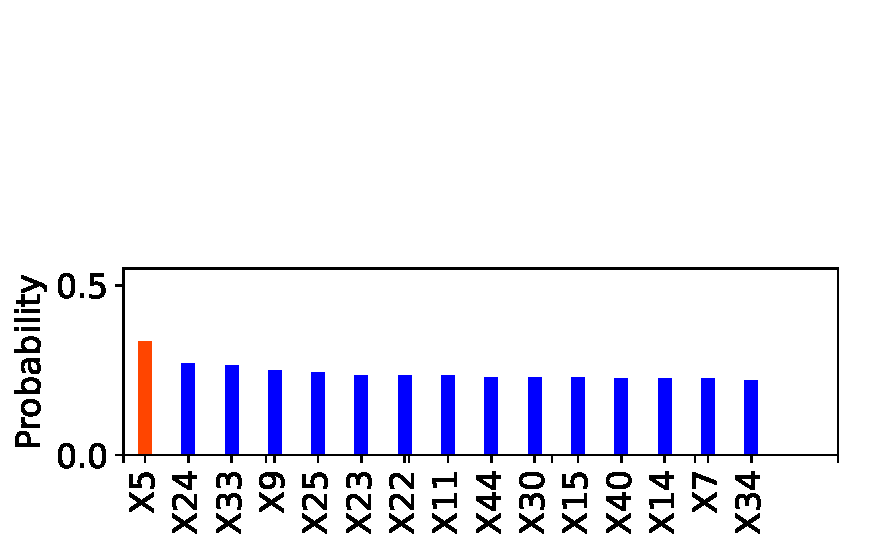
\includegraphics[width=0.25\paperwidth]{acc_plot_top20_ic_25_False_lars-crop.pdf}}
  %
  \subfloat[\label{fig:solar_ic_type-II2}$\omega = 1/3,\;\mu\left(F\right)=2/3$, lasso]
  {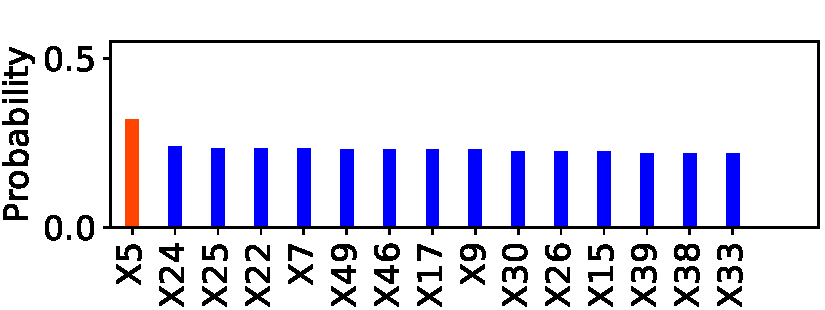
\includegraphics[width=0.25\paperwidth]{acc_plot_top20_ic_33_False_lars-crop.pdf}}
  %
  \subfloat[\label{fig:solar_ic_type-II3}$\omega = 1/2,\;\mu\left(F\right)=1$, lasso]
  {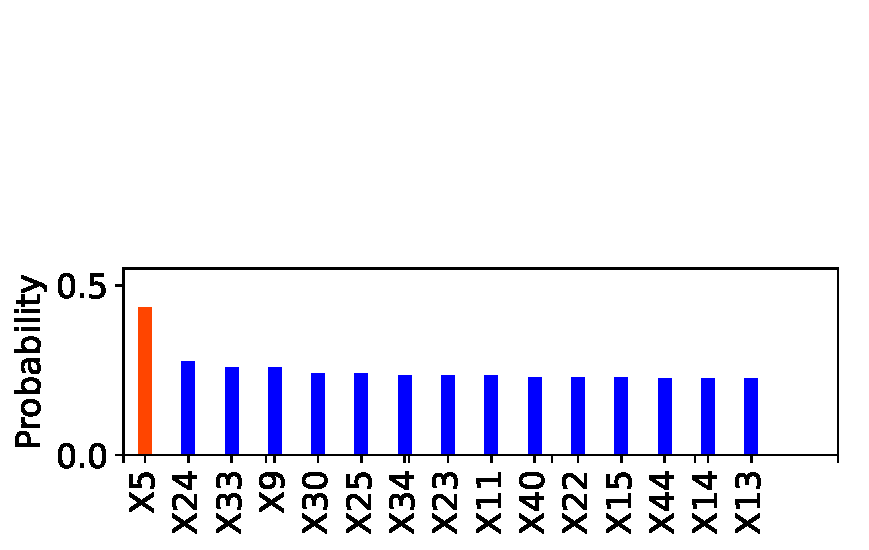
\includegraphics[width=0.25\paperwidth]{acc_plot_top20_ic_5_False_lars-crop.pdf}}

  \subfloat[\label{fig:solar_ic_type-II7}$\omega = 1/4,\;\mu\left(F\right)=1/2$, solar]
  {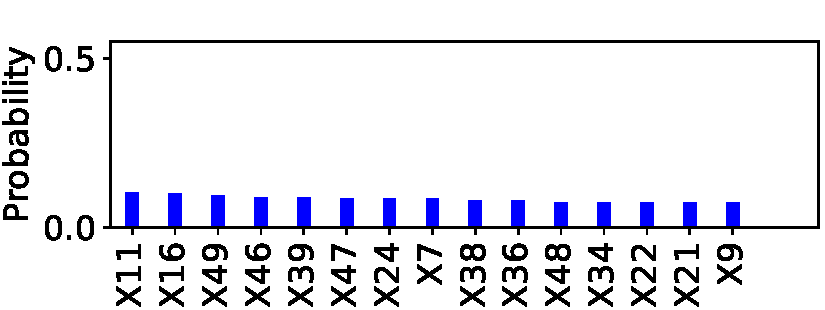
\includegraphics[width=0.25\paperwidth]{acc_plot_top20_ic_25_False_solar-crop.pdf}}
  %
  \subfloat[\label{fig:solar_ic_type-II8}$\omega = 1/3,\;\mu\left(F\right)=2/3$, solar]
  {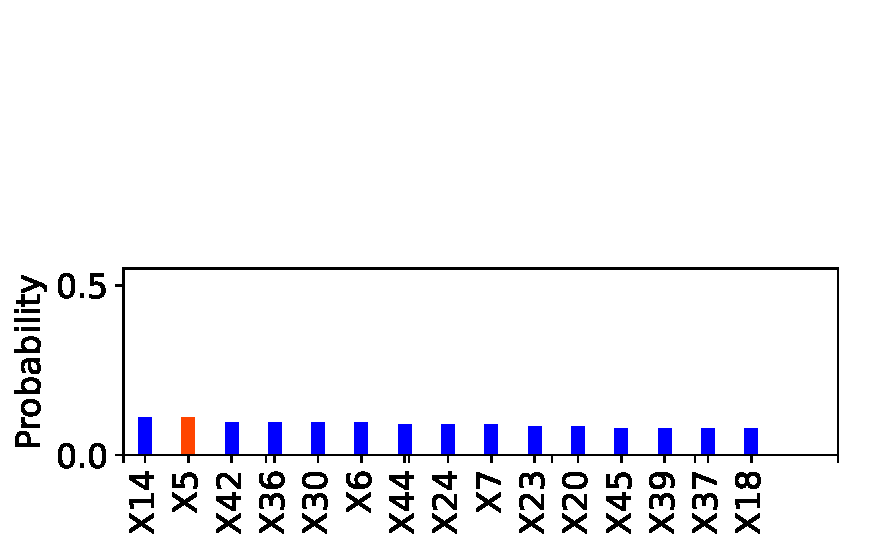
\includegraphics[width=0.25\paperwidth]{acc_plot_top20_ic_33_False_solar-crop.pdf}}
  %
  \subfloat[\label{fig:solar_ic_type-II9}$\omega = 1/2,\;\mu\left(F\right)=1$, solar]
  {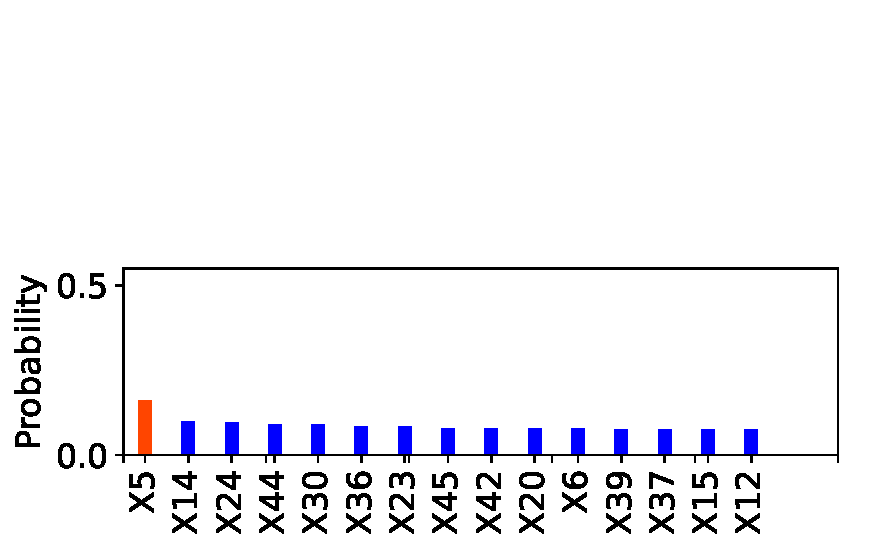
\includegraphics[width=0.25\paperwidth]{acc_plot_top20_ic_5_False_solar-crop.pdf}}
  %
  \caption{Probability of including redundant variables (top 15) in simulation~2 ($\mathbf{x}_5$ in orange).}
  \label{fig:solar_ic_type-II}
  %
\end{figure}

Figure~\ref{fig:solar_ic_type-II} displays the simulation~2 results. When $\mu \left( F \right) = 1/2$, lasso wrongly includes $\mathbf{x}_5$ with probability $0.25$. By contrast, $\mathbf{x}_5$ does not crack the top-10 list for solar, implying that the corresponding probability remains below $0.1$. When $\mu \left( F \right)$ increases to $2/3$, the probability that lasso includes $\mathbf{x}_5$ increases to around $0.3$, standing out from the other 9 variables. When $\mu \left( F \right)$ jumps to $1$ in the population and strong IRC is violated, the probability that lasso includes $\mathbf{x}_5$ rises to almost $0.5$. Despite the increase in $\mu\left(F\right)$, the probability that solar includes $\mathbf{x}_5$ is always below $0.1$. The results illustrate that solar is more robust to different settings of the IRC.

\subsection{Simulation 3: computation and performance improvements over lasso-related subsampling variable selection}

The lasso ensemble repeats lasso multiple times on the data, producing the averaged (or accumulated) results of all the repetitions. In simulation~3, we show that replacing lasso with solar improves the variable selection performance and substantially reduces the computation load.

An ensemble system may be constructed via the bootstrap or boosting. The bootstrap ensemble (also called stability selection by \citet{meinshausen2010stability}) evaluates lasso on many subsamples, choosing variables that are selected in the majority of subsamples. The boosting ensemble runs multiple iterations of lasso on the full sample, feeding variables selected by lasso to the next iteration. Both methods require running lasso multiple times. However, previous research suggests the bootstrap ensemble may be more stable and robust than boosting. In one realization, if the boosting ensemble wrongly dropped an informative variable at the first iteration, all subsequent iterations suffered from the same error. By contrast, if an informative variable is dropped in a subsample, the bootstrap ensemble may still select the variable as long as it is picked up in most of the other subsamples. Thus, we focus on the bootstrap ensemble in simulation~3 and use bolasso \citep{bach2008bolasso} as the competitor to solar.

\citet{bach2008bolasso} proposes two bolasso algorithms: bolasso-H and bolasso-S. Bolasso-H selects only variables that are selected in all subsamples, i.e., the subsample selection frequency threshold, $f=1$. Bolasso-S selects variables that are selected in 90\% of the subsamples ($f=0.9$). In simulation~3, we use both as the competitors. \citet{bach2008bolasso} finds that it is always beneficial, in terms of selection and prediction, to generate more subsamples in bolasso. As such, we set the number of subsamples in bolasso to $256$, the maximum in the \citet{bach2008bolasso} simulations.

The bootstrap solar ensemble (bsolar) runs solar on each subsample and computes the selection frequency for each variable across subsamples. To ensure that any performance improvement is due to replacing lasso with solar in the bootstrap ensemble, bsolar and bolasso use the same $f$. Thus, we evaluate 2~versions of bsolar: bsolar-H ($f=1$) and bsolar-S ($f=0.9$). \footnote{If the sample comes with small $n$ or large noise level, we may reserve part of the data as a validation set for the bootstrap ensemble, choosing the optimal $f$ by minimizing the validation error.} To denote the number of subsamples clearly, we use the notation bsolar-$m$H and bsolar-$m$S, where $m$ is the number of subsamples used to compute the selection frequency. To compare the performance of bolasso, bsolar and solar, we use the same DGP, Python random seeds (for data generation), and $p/n$ settings as simulation~1.

\subsubsection*{Comparison of computation load and subsample selection frequency}

With ultrahigh-dimensional data, maintaining a feasible computation load is critical. Since the computation load of least-angle regression on a given sample is fixed, we may use the number of least-angle regressions required by solar and $K$-fold, cross-validated least-angle regression for lasso (lasso for short) to approximate the respective computation loads. For comparison purposes, we compute solar with $K$ subsamples and lasso with $K$-fold cross-validation. As shown in Algorithm~\ref{algo:APE-lar}, we need to compute one unconstrained least angle regression for solar on each subsample $(X^k, Y^k)$, implying we need to estimate $K$ unconstrained least-angle regressions to compute $\widehat{q}$ and one to compute $c^*$ for variable selection. Lasso requires computing $K$ least angle regressions to optimize the tuning parameter $t$ and, given the optimal tuning parameter, one extra least angle regression on the full sample to select variables. Thus, the computation load for solar is approximately the same as for lasso.

Due to the equality of the computataion load between solar and lasso, in this round of simulations, differences in computation load are due primarily to subsample repetition. So we measure computation load by \emph{the number of subsample repetitions (SR) required by the competitors}. Thus, solar and lasso have a computation load of $1$ SR, bolasso has a load of $256$ SR, and bsolar-3/5/10 a load of $3/5/10$ SR.

\begin{table}[h]
	\centering
	\caption{Subsample selection frequency for bolasso and bsolar-10.}
	\label{table:subsample_select_freq}
    \captionsetup[subfloat]{font=normalsize}
	\subfloat[bolasso (subsample selection frequency $\geqslant 0.67$)]{%
    \label{table:subsample_select_freq_1}
			\renewcommand{\arraystretch}{0.7}
			\begin{tabular}{cl}
				\toprule
				frequency & variables \\
				\midrule
				$\geqslant 1.00$ & $\mathbf{x}_4, \mathbf{x}_3, \mathbf{x}_2, \mathbf{x}_1, \mathbf{x}_0$ \\
				$\geqslant 0.88$ & $\mathbf{x}_4, \mathbf{x}_3, \mathbf{x}_2, \mathbf{x}_1, \mathbf{x}_0, \mathbf{x}_{28}$ \\
				$\geqslant 0.84$ & $\mathbf{x}_4, \mathbf{x}_3, \mathbf{x}_2, \mathbf{x}_1, \mathbf{x}_0, \mathbf{x}_{28}, \mathbf{x}_{71}$\\
				$\geqslant 0.76$ & $\mathbf{x}_4, \mathbf{x}_3, \mathbf{x}_2, \mathbf{x}_1, \mathbf{x}_0, \mathbf{x}_{28}, \mathbf{x}_{71}, \mathbf{x}_{91}$\\
				$\geqslant 0.70$ & $\mathbf{x}_4, \mathbf{x}_3, \mathbf{x}_2, \mathbf{x}_1, \mathbf{x}_0, \mathbf{x}_{28}, \mathbf{x}_{71}, \mathbf{x}_{91}, \mathbf{x}_{94}$\\
				$\geqslant 0.69$ & $\mathbf{x}_4, \mathbf{x}_3, \mathbf{x}_2, \mathbf{x}_1, \mathbf{x}_0, \mathbf{x}_{28}, \mathbf{x}_{71}, \mathbf{x}_{91}, \mathbf{x}_{94}, \mathbf{x}_{70}, \mathbf{x}_{40}$\\
				$\geqslant 0.67$ & $\mathbf{x}_4, \mathbf{x}_3, \mathbf{x}_2, \mathbf{x}_1, \mathbf{x}_0, \mathbf{x}_{28}, \mathbf{x}_{71}, \mathbf{x}_{91}, \mathbf{x}_{94}, \mathbf{x}_{70}, \mathbf{x}_{40}, \mathbf{x}_{90}$                  \\
				\bottomrule
		\end{tabular}
	}

    \captionsetup[subfloat]{font=normalsize,width=0.6\textwidth}
	\subfloat[bsolar-10 (subsample selection frequency $> 0$)]{%
    \label{table:subsample_select_freq_2}
			\renewcommand{\arraystretch}{0.7}
			\begin{tabular}{cl}
				\toprule
				frequency & variables \\
				\midrule
				$\geqslant 1.00$ & $\mathbf{x}_4, \mathbf{x}_3, \mathbf{x}_2, \mathbf{x}_1, \mathbf{x}_0$ \\
				$\geqslant 0.10$ & $\mathbf{x}_4, \mathbf{x}_3, \mathbf{x}_2, \mathbf{x}_1, \mathbf{x}_0, \mathbf{x}_{91}, \mathbf{x}_{71}$ \\
				\bottomrule
		\end{tabular}
	}
\end{table}

We know from simulation~1 that lasso is prone to selecting a number of redundant variables. Consequently, bolasso requires many subsample repetitions to distinguish informative from redundant variables. By contrast, bsolar requires fewer repetitions due to the sparsity and accuracy of solar. As shown in Table~\ref{table:subsample_select_freq}, bsolar is more efficient and accurate than bolasso. Table~\ref{table:subsample_select_freq_1} shows the subsample selection frequency list from 256 subsamples for one bolasso realization with $p/n=100/200$. Even after 256 subsample repetitions, bolasso is not able clearly to separate informative from redundant variables: the frequency discrepancy between the highest-ranking redundant ($\mathbf{x}_{28}$) and the lowest-ranking informative variable ($\mathbf{x}_0$) is only $0.12$. By contrast, for bsolar-10, the frequency discrepancy between the highest-ranking redundant ($\mathbf{x}_{91}$) and the lowest-ranking informative variable ($\mathbf{x}_0$) is $0.9$. Thus, for a given selection frequency threshold, bsolar-10 is much less likely to include redundant variables.

More importantly, the bolasso computation load of 256 SR is more than 25 times the bsolar-10 load of 10 SR. Thus, the solar ensemble improves the subsample selection frequency list while reducing the bolasso subsample repetitions by 96\%. We know from the \citet{bach2008bolasso} result that increasing the number of subsamples in bolasso may increase the discrepancy between the lowest ranked informative and the highest ranked redundant variables. However, increasing the subsample repetitions substantially raises the computation load of bolasso in high-dimensional spaces, making bsolar-10 even more computationally preferable.

\subsubsection*{Comparison of accuracy and sparsity}

Using the same simulation setting, DGP, and $p/n$ scenarios as simulation~1, we next show that replacing lasso with solar in the ensemble improves variable selection sparsity. The competitors to bolasso are bsolar-3/5/10.\footnote{In large-scale simulations, we find that the optimal number of subsamples for bsolar is around $10$. More than $10$ subsamples raises the computation load without any substantial performance improvement.} All the simulations in Table~\ref{table:subsample_select_freq} return the same results for bsolar-H ($f=1$) and bsolar-S ($f=0.9$). Thus, bsolar-H and -S are reported jointly in Tables~\ref{table:sim_3_info} and~\ref{table:sim_3}.

\begin{table}[h]
	\small
	\centering
	\caption{Probability of including informative variables in simulation~3 (two decimal places).} \label{table:sim_3_info}
	  \renewcommand{\arraystretch}{0.7}
		\begin{tabular}{ll.........}
			\toprule
			&           & \multicolumn{3}{c}{$p/n \rightarrow 0$} & \multicolumn{3}{c}{$p/n \rightarrow 1$} & \multicolumn{3}{c}{$\log(p)/n\rightarrow0$}\\
			\cmidrule(l){3-5} \cmidrule(l){6-8} \cmidrule(l){9-11}
			&           & \multicolumn{1}{c}{$\frac{100}{100}$} & \multicolumn{1}{c}{$\frac{100}{150}$} & \multicolumn{1}{c}{$\frac{100}{200}$} & \multicolumn{1}{c}{$\frac{150}{100}$} & \multicolumn{1}{c}{$\frac{200}{150}$} & \multicolumn{1}{c}{$\frac{250}{200}$} & \multicolumn{1}{c}{$\frac{400}{200}$} & \multicolumn{1}{c}{$\frac{800}{400}$} & \multicolumn{1}{c}{$\frac{1200}{600}$}\\
			\midrule
			$\Pr(\mbox{select }\mathbf{x}_0)$
      & bsolar-3S/3H   & 1 & 1 & 1 & 1    & 1 & 1 & 1 & 1 & 1 \\
			& bsolar-5S/5H   & 1 & 1 & 1 & 1    & 1 & 1 & 1 & 1 & 1 \\
      & bsolar-10S/10H & 1 & 1 & 1 & 0.99 & 1 & 1 & 1 & 1 & 1 \\
			& bolasso-S      & 1 & 1 & 1 & 1    & 1 & 1 & 1 & 1 & 1 \\
			& bolasso-H      & 1 & 1 & 1 & 1    & 1 & 1 & 1 & 1 & 1 \\
			\\[-8pt]
			$\Pr(\mbox{select }\mathbf{x}_1)$
      & bsolar-3S/3H   & 1 & 1 & 1 & 1 & 1 & 1 & 1 & 1 & 1 \\
      & bsolar-5S/5H   & 1 & 1 & 1 & 1 & 1 & 1 & 1 & 1 & 1 \\
      & bsolar-10S/10H & 1 & 1 & 1 & 1 & 1 & 1 & 1 & 1 & 1 \\
			& bolasso-S      & 1 & 1 & 1 & 1 & 1 & 1 & 1 & 1 & 1 \\
			& bolasso-H      & 1 & 1 & 1 & 1 & 1 & 1 & 1 & 1 & 1 \\
			\\[-8pt]
			$\Pr(\mbox{select }\mathbf{x}_2)$
      & bsolar-3S/3H   & 1 & 1 & 1 & 1 & 1 & 1 & 1 & 1 & 1 \\
      & bsolar-5S/5H   & 1 & 1 & 1 & 1 & 1 & 1 & 1 & 1 & 1 \\
      & bsolar-10S/10H & 1 & 1 & 1 & 1 & 1 & 1 & 1 & 1 & 1 \\
			& bolasso-S      & 1 & 1 & 1 & 1 & 1 & 1 & 1 & 1 & 1 \\
			& bolasso-H      & 1 & 1 & 1 & 1 & 1 & 1 & 1 & 1 & 1 \\
			\\[-8pt]
			$\Pr(\mbox{select }\mathbf{x}_3)$
      & bsolar-3S/3H   & 1 & 1 & 1 & 1 & 1 & 1 & 1 & 1 & 1 \\
			& bsolar-5S/5H   & 1 & 1 & 1 & 1 & 1 & 1 & 1 & 1 & 1 \\
      & bsolar-10S/10H & 1 & 1 & 1 & 1 & 1 & 1 & 1 & 1 & 1 \\
			& bolasso-S      & 1 & 1 & 1 & 1 & 1 & 1 & 1 & 1 & 1 \\
			& bolasso-H      & 1 & 1 & 1 & 1 & 1 & 1 & 1 & 1 & 1 \\
			\\[-8pt]
			$\Pr(\mbox{select }\mathbf{x}_4)$
      & bsolar-3S/3H   & 1 & 1 & 1 & 1 & 1 & 1 & 1 & 1 & 1 \\
      & bsolar-5S/5H   & 1 & 1 & 1 & 1 & 1 & 1 & 1 & 1 & 1 \\
      & bsolar-10S/10H & 1 & 1 & 1 & 1 & 1 & 1 & 1 & 1 & 1 \\
			& bolasso-S      & 1 & 1 & 1 & 1 & 1 & 1 & 1 & 1 & 1 \\
			& bolasso-H      & 1 & 1 & 1 & 1 & 1 & 1 & 1 & 1 & 1 \\
			\bottomrule
	\end{tabular}
\end{table}

Table~\ref{table:sim_3_info} summarizes the accuracy results. Recall the DGP has 5~informative variables with population regression coefficients absolute value (aka signal strength) $\left[2, 3, 4, 5, 6 \right]$. For the most part, all the competitors are able to distinguish informative from redundant variables, selecting each informative variable with probability $1$ in most $p/n$ scenarios. While bsolar-10S and bsolar-10H occasionally drop $\mathbf{x}_0$ at $p/n=150/100$, it is of little consequence overall since $\Pr(\mbox{select }\mathbf{x}_0)=0.99$.

Table~\ref{table:sim_3} summarizes the sparsity results. By and large, the bsolar competitors outperform bolasso-S in terms of sparsity. As $p/n\rightarrow0$ or $\rightarrow1$, bsolar-$10$ sparisty is virtually the same as bolasso-H. A similar tendency is found when $\log(p)/n \rightarrow 0$.

\begin{table}[h]
	\small
	\centering
	\caption{Number of variables selected in simulation~3.\label{table:sim_3}}
	\resizebox{1\textwidth}{!}{%
		\renewcommand{\arraystretch}{0.7}
		\begin{tabular}{ll.........}
			\toprule
			&           & \multicolumn{3}{c}{$p/n\rightarrow0$}    & \multicolumn{3}{c}{$p/n\rightarrow1$} & \multicolumn{3}{c}{$\log(p)/n\rightarrow0$} \\
			\cmidrule(lr){3-5}\cmidrule(lr){6-8}\cmidrule(lr){9-11}
			&           & \multicolumn{1}{c}{$\frac{100}{100}$} & \multicolumn{1}{c}{$\frac{100}{150}$} & \multicolumn{1}{c}{$\frac{100}{200}$} & \multicolumn{1}{c}{$\frac{150}{100}$} & \multicolumn{1}{c}{$\frac{200}{150}$} & \multicolumn{1}{c}{$\frac{250}{200}$} & \multicolumn{1}{c}{$\frac{400}{200}$} & \multicolumn{1}{c}{$\frac{800}{400}$} & \multicolumn{1}{c}{$\frac{1200}{600}$} \\
			\midrule
			mean
      & bsolar-3S/3H   & 5.45 & 5.16 & 5.20 & 5.47 & 5.17 & 5.07 & 5.16 & 5.25 & 5.46 \\
      & bsolar-5S/5H   & 5.14 & 5.04 & 5.10 & 5.15 & 5.04 & 5.04 & 5.06 & 5.12 & 5.12 \\
			& bsolar-10S/10H & 5.06 & 5.01 & 5    & 5.03 & 5    & 5    & 5.01 & 5.01 & 5.03 \\
			& bolasso-S      & 5.46 & 6.09 & 6.60 & 5.39 & 5.72 & 6.06 & 5.66 & 6.72 & 7.69 \\
			& bolasso-H      & 5    & 5.02 & 5.01 & 5    & 5.01 & 5    & 5    & 5    & 5.02 \\
			\\[-8pt]
			median
      & bsolar-3S/3H   & 5 & 5 & 5 & 5 & 5 & 5 & 5 & 5 & 6 \\
      & bsolar-5S/5H   & 5 & 5 & 5 & 5 & 5 & 5 & 5 & 5 & 5 \\
			& bsolar-10S/10H & 5 & 5 & 5 & 5 & 5 & 5 & 5 & 5 & 5 \\
			& bolasso-S      & 5 & 6 & 6 & 6 & 5 & 6 & 5 & 6 & 8 \\
			& bolasso-H      & 5 & 5 & 5 & 5 & 5 & 5 & 5 & 5 & 5 \\
			\\[-8pt]
			\bottomrule
	\end{tabular}}
\end{table}

\subsubsection*{Comparison of runtime}

It turns out, solar also substantially reduces the runtime of the bootstrap ensemble. To ensure that each CPU core is assigned the same amount of computation and the CPU frequency is at a maximum, we follow the recommendations of the \texttt{Sci-kit learn} package and design a high-level parallel architecture, denoted \emph{Joblib parallel}.

\begin{table}[h]
  \centering
  \caption{Average runtime (seconds) for solar, bsolar, and bolasso over 30 repetitions.\label{table:sim_3_comp}}
  \resizebox{1\textwidth}{!}{%
  \renewcommand{\arraystretch}{0.7}
  \begin{tabular}{rrrrrrrrrrr}
    \toprule
    &
    & \multicolumn{3}{c}{$p/n\rightarrow0$}
    & \multicolumn{3}{c}{$p/n\rightarrow1$}
    & \multicolumn{3}{c}{$\log(p)/n\rightarrow0$} \\
	\cmidrule(lr){3-5}\cmidrule(lr){6-8}\cmidrule(lr){9-11}
    & SR & $\frac{100}{100}$ & $\frac{100}{150}$ & $\frac{100}{200}$ & $\frac{150}{100}$ & $\frac{200}{150}$ & $\frac{250}{200}$ & $\frac{400}{200}$ & $\frac{800}{400}$ & $\frac{1200}{600}$ \\
    \midrule
    solar + hold out                                 & 1   & 0.09  & 0.10  & 0.11  & 0.09  & 0.12   & 0.16   & 0.19   & 0.92   & 1.62 \\
    bsolar-3                                         & 3   & 0.33  & 0.22  & 0.24  & 0.19  & 0.27   & 0.35   & 0.46   & 1.07   & 2.40 \\
    bolasso (joblib parallel)                        & 256 & 6.71  & 11.88 & 9.37  & 7.22  & 13.05  & 24.39  & 38.44  & 608.94 & 1819.51 \\
    bolasso (built-in parallel)                      & 256 & 6.78  & 11.94 & 18.67 & 7.50  & 16.25  & 25.75  & 46.41  & 636.29 & 1731.38 \\
    bolasso (coordinated descent, built-in parallel) & 256 & 16.99 & 61.34 & 61.10 & 33.60 & 166.99 & 196.50 & 240.36 & 632.26 & 1412.01 \\
    \bottomrule
    \end{tabular}}
\end{table}

Since bsolar and bolasso are very similar in terms of their computation procedures, they are coded similarly to make the comparison fair. The only substantive code difference lies in the computation of subsample selection frequency.\footnote{See Read\_Me\_First.html in the supplementary file for more detail.} Thus, runtime differences below are due to the reduction in subsample repetitions from the solar ensemble. To avoid any possibility that \emph{Joblib parallel} is too demanding for bolasso, we also compute bolasso using the built-in \texttt{Sci-kit learn} parallel scheme (denoted as \emph{built-in parallel}), which is optimized for lasso.

Table~\ref{table:sim_3_comp} summarizes average runtime in 200 repetitions on Dell all-in-one with Intel i7-10700 CPU and 16GB RAM. The first three rows of Table~\ref{table:sim_3_comp} show runtimes using \emph{Joblib parallel} and the last row shows runtimes using \emph{built-in parallel}. As it turns out, \emph{built-in parallel} is marginally faster only at $\log(p)/n \rightarrow 0$. Overall, both \emph{solar + hold out} and bsolar-3 have much shorter runtimes than bolasso. Due to the long-time and heavy (90\% to 100\%) CPU load of bolasso, the CPU frequency is often automatically reduced to reduce the heat generated and possible damage to the chip. By contrast, neither \emph{solar + hold out} nor bsolar trigger dynamic frequency scaling and, as a result, the runtime differences become even more pronounced as $p$ and $n$ increase. We also compute \emph{solar + hold out}, bsolar and bolasso on an i9-9900K CPU, report the corresponding runtime in the supplementary files. We find that the the runtimes of \emph{solar + hold out} and bsolar are stable across different CPUs and platforms. By contrast, bolasso amplifies any runtime change for lasso and least-angle regression due to the 256 repetitions, varying its runtime significantly across different hardware settings and Python environments. 

More interestingly, we find in our bolasso simulation that, unlike \citet{friedman2007pathwise}, the coordinate descent solver is almost at the same speed as least angle regression; with smaller $n$ and $p$, the least angle regression is actually much faster. After carefully checking the code, Intel MKL C++ library and the source code in Python, we find that it is not surprising since (i) compared to the standard BLAS and LAPACK for Fortran and C++ 14 years ago, the modern Intel MKL C++ library is heavily optimized and can be much 15-30 times faster on matrix operations like dot multiplication, descomposition and inversion; \footnote{ See \url{https://towardsdatascience.com/is-your-numpy-optimized-for-speed-c1d2b2ba515} for detailed comparison} (ii) the current CPU parallel scheme heavily rewards light-weight computations;\footnote{ Using technologies like Turbo boost, Intel CPU can lower the frequency and voltage of other cores while significantly increase the frequncy in one or two cores. As a result, light-weight computations like solar and bsolar only utilize 1 or 2 cores and, hence, can be done even quicker, compared to the old CPU parallel schemes} (iii) unlike \citet{friedman2007pathwise} comparing Fortran speed with R speed, we compare coordinate descent and least angle regression in the same Python platform with well optimized Python and C++ libraries; (iv) the DGP, $n$, $p$ settings are different. When $p/n$ is drastically large (say $p/n=200$) and both $p$ and $n$ are huge, coordinate descent solver may show its computation advantage over least-angle regression for lasso. However, due to the 256 lasso repetition, it may be difficult to come on-par with bsolar. Lastly, alongside with least-angle regression, coordinate descent can also be used to compute solar. The key for solar is to compute the average $L_0$ path, which is computed using least-angle regression in Algorithm~\ref{algo:APE-lar}. Since the lasso coefficient path can also be computed using coordinate descent, so does the average $L_0$ path. Hence, when $p/n$ is drastically large (say $p/n=200$) and both $p$ and $n$ are huge, coordinate descent solver can be used to solve bsolar and solar as well.

\subsubsection*{Comparison summary}

In summary, with very similar accuracy and sparsity, bsolar and \emph{solar + hold out} generate large reductions in computation load and runtime. This is potentially very useful in ultrahigh dimensional applications, such as natural language processing and picture recognition, where often $p>10^6$. Indeed, the solar ensemble results can potentially be further improved by adopting the \cite{tibshirani2015general} procedure, which outperforms other optimization techniques (e.g., warm-start cylindrical coordinate descent and warm-start Frank-Wolfe methods) in terms of runtime and statistical performance in group-structured learning, matrix completion, image denoising and other applications.

Despite a slightly longer runtime, bsolar has advantages over \emph{solar + hold out}. Firstly, bsolar has a higher probability of selecting each informative variable while an accurate hold-out average requires sufficient sample points for testing. Table~\ref{table:sim_3_info} shows that, despite the signal strength, a hold-out average may occasionally drop an informative variable with limited residual degrees of freedom. Secondly, bsolar has slightly better sparsity when $\log(p)/n \rightarrow 0$. Thirdly, thanks to the bootstrap, bsolar is robust to empirical issues that arise when the classical OLS assumptions are violated, unlike \emph{solar + hold out} where the accuracy of t, F, or $\chi^2$ tests may be affected. Lastly, bsolar is computationally straightforward and does not require asymptotic distribution analysis. In complicated ensemble learning applications, it may not be straightforward to find simple and efficient test statistics for the hold-out average to screen each $\mathbf{x}_i$.

\section{Real-world data: Sydney house price prediction\label{section:application}}

To demonstrate that the improvements from solar are empirically feasible, we apply solar to real-world data. In the context of the simulations above, the real-world data reflect both the $p/n\rightarrow0$ scenarios of simulation~1 and the high multicollinearity and complicated dependence structures of simulation~2. As such, the data reflect the challenging IRC settings, complicated dependence structures, and grouping effects typical of data in the social sciences.

The sample is assembled from more than 10 different databases: Sydney, Australia, real estate market transaction data for 11,974 houses sold in 2010, including price and house attribute information (property address, bedrooms, bathrooms, car spaces, etc.), matched to 2011 census data by Statistical Area Level 1 (the smallest census area in Australia, comprising at most 200 people or 60 households), 2010 and 2011 crime data by suburb, 2010 GIS data (extracted from a geo-spatial topological database, a climate database, a pollution database, and the Google Maps database), 2009 primary and secondary school data, and 2010 Sydney traffic and public transport data (bus routes, train stations, and ferry wharfs). Following the hedonic pricing approach (see \citet{sirmans2005hedonic} for a review), we predict house price with a linear model.

Using an ensemble of Bayes network learning algorithms for data clearning, we purge variables with both very low conditional and unconditional correlations to house price. The remaining variables are listed in the first column of Table~\ref{table:house_variable}.\footnote{Due to 200GB size of the database, we only include the data for these variables in the supplementary file.} The 57 variables fall into 5 categories: house attributes, distance to key locations (public transport, shopping, etc.), neighbourhood socio-economic data, localized administrative and crime data, and local school quality. Pairwise correlations among all 57 covariates indicate, not surprisingly, severe multicollinearity and grouping effects, implying a harsh IRC setting.\footnote{Correlations and IRC are also reported in supplementary files.} Thus, heuristically increasing the value of the tuning parameter in lasso-type estimators (e.g., using the one-sd or the `elbow' rule) is unlikely to be useful since it may trigger further grouping effects and the random dropping of variables.

Table~\ref{table:house_variable} shows the selection comparison across the elastic net, lasso, and solar. With all variables in linear form, both lasso and elastic net lose sparsity due to the complicated dependence structures and severe multicollinearity in the data, consistent with \citet{jia2010model}. By contrast, solar returns a much sparser model, with only $9$ variables selected from $57$. A very similar result can be found with the variables in log form, hinting that solar possesses superior selection sparsity and robustness to a change in functional form. More importantly, solar variable selection outperforms the lasso-type estimators in terms of the balance between sparsity and prediction power. While pruning most of the variables from the elastic net and lasso selections, solar reduces the post-selection regression $\mathrm{R}^2$ by only 3-5\%. In the supplementary file, we also perform a hold-out average method to avoid the possibility that the `p-value overfitting' issue also affects the direct post-selection OLS $R^2$. However, there is no concern in this sample because $p/n=57/11,974$. This confirms that, from the perspective of prediction, solar successfully identifies the most important variables in the database.

%%%%%%%%%%%%%%%%%%%%%%%%%%%%%%%%%%
%%%%%%%%%%% Conclusion %%%%%%%%%%%
%%%%%%%%%%%%%%%%%%%%%%%%%%%%%%%%%%

\section{Conclusion}

In this paper we offer a new least-angle regression algorithm for high-dimensional data called solar (for subsample-ordered least-angle regression). We show that solar yields substantial improvements over lasso in terms of the sparsity, stability, accuracy, and robustness of variable selection. We also illustrate the improvements relative to lasso ensembles from solar ensembles in terms of variable selection accuracy, sparsity and computation load.

Detection of weak signals is a small weakness evident in solar, although relative to the lasso competitor the difference is very slight. Nonetheless, we are working on an extension to solar, the double-bootstrap solar (DBsolar), which, if early results are any indication, promises to enable solar accurately to detect variables with weak signals.

Lastly, the speed of solar will likely benefit from recoding in C++. Specifically, Python is not as advanced as C++ in concurrency, multi-processes and multi-threads while \texttt{solarpy} and \texttt{Joblib} require a highly efficient interpreter. Especially for cases with $p>1\times10^6$ (typical in text mining, computer vision, and natural language processing), coding solar in GPU-based C++ will probably further reduce runtime by a factor of $10$. We are working on a GPU version of solar. For details, see the Read\_Me\_First.html in the supplementary file.

\subsection*{Supplementary material}

\noindent
\textbf{Supplementary\_file.zip:} Python code, general description, detailed explanations, raw Python log files, and numerical results for sections~2, 3, and~4.

%%%%%%%%%%%%%%%%%%%%%%%%%%%%%%%%%%
%%%%%%%%%%% References %%%%%%%%%%%
%%%%%%%%%%%%%%%%%%%%%%%%%%%%%%%%%%

\bibliographystyle{elsarticle-harv}
\bibliography{ref/CVrefs}

\begin{table}[H]
  %
  \centering
  %
  \small
  %
  \caption{Variable selection results for linear and log house price models. \label{table:house_variable}}
  %
  \resizebox*{!}{0.95\textheight}{%
  \renewcommand{\arraystretch}{0.6}
  \begin{tabular}{@{}ll@{\extracolsep{6pt}}c@{\extracolsep{-2pt}}c@{\extracolsep{6pt}}c@{\extracolsep{-2pt}}c@{\extracolsep{6pt}}c@{\extracolsep{-2pt}}c@{}}
    %
    \toprule
    %
            &             & \multicolumn{2}{c}{elastic net}
                          & \multicolumn{2}{c}{lasso}
                          & \multicolumn{2}{c}{solar} \\
                          \cline{3-4} \cline{5-6} \cline{7-8} \\[-7pt]
    %
    Variable & Description& \multicolumn{1}{c}{linear}
                          & \multicolumn{1}{c}{log}
                          & \multicolumn{1}{c}{linear}
                          & \multicolumn{1}{c}{log}
                          & \multicolumn{1}{c}{linear}
                          & \multicolumn{1}{c}{log} \\
    %
    \midrule
    %
    Bedrooms           & property, number of bedrooms             & \checkmark  & \checkmark  & \checkmark  & \checkmark  & \checkmark & \checkmark  \\
    %
    Baths              & property, number of bathrooms            & \checkmark  & \checkmark  & \checkmark  & \checkmark  & \checkmark & \checkmark  \\
    %
    Parking            & property, number of parking spaces       & \checkmark  & \checkmark  & \checkmark  & \checkmark  & \checkmark & \checkmark  \\
    %
    AreaSize           & property, land size                      & \checkmark  & \checkmark  & \checkmark  & \checkmark  &   &    \\ \midrule
    %
    Airport            & distance, nearest airport                & \checkmark  & \checkmark  & \checkmark  & \checkmark  &   &    \\
    %
    Beach              & distance, nearest beach                  & \checkmark  & \checkmark  & \checkmark  & \checkmark  & \checkmark & \checkmark  \\
    %
    Boundary           & distance, nearest suburb boundary        & \checkmark  & \checkmark  & \checkmark  & \checkmark  &   &    \\
    Cemetery           & distance, nearest cemetery               & \checkmark  &             & \checkmark  &    &   &    \\
    %
    Child care         & distance, nearest child-care centre      & \checkmark  & \checkmark  & \checkmark  & \checkmark  &   & \checkmark  \\
    %
    Club               & distance, nearest club                   & \checkmark  & \checkmark  & \checkmark  & \checkmark  &   &    \\
    %
    Community facility & distance, nearest community facility     & \checkmark  & \checkmark  &    &    &   &    \\
    %
    Gaol               & distance, nearest gaol                   & \checkmark  & \checkmark  &    &    & \checkmark & \checkmark  \\
    %
    Golf course        & distance, nearest golf course            & \checkmark  & \checkmark  & \checkmark  & \checkmark  &   &    \\
    %
    High               & distance, nearest high school            & \checkmark  & \checkmark  & \checkmark  & \checkmark  &   &    \\
    %
    Hospital           & distance, nearest general hospital       & \checkmark  & \checkmark  &    & \checkmark  &   &    \\
    %
    Library            & distance, nearest library                & \checkmark  &             & \checkmark  &    &   &    \\
    %
    Medical            & distance, nearest medical centre         & \checkmark  & \checkmark  &    & \checkmark  &   &    \\
    %
    Museum             & distance, nearest museum                 & \checkmark  & \checkmark  & \checkmark  & \checkmark  &   &    \\
    %
    Park               & distance, nearest park                   & \checkmark  & \checkmark  & \checkmark  &    &   &    \\
    %
    PO                 & distance, nearest post office            & \checkmark  & \checkmark  &    & \checkmark  &   &    \\
    %
    Police             & distance, nearest police station         & \checkmark  & \checkmark  & \checkmark  & \checkmark  &   &    \\
    %
    Pre-school         & distance, nearest preschool              & \checkmark  & \checkmark  & \checkmark  & \checkmark  &   &    \\
    %
    Primary            & distance, nearest primary school         & \checkmark  & \checkmark  & \checkmark  & \checkmark  &   &    \\
    %
    Primary High       & distance, nearest primary-high school    & \checkmark  & \checkmark  & \checkmark  & \checkmark  &   &    \\
    %
    Rubbish            & distance, nearest rubbish incinerator    & \checkmark  & \checkmark  & \checkmark  &    &   &    \\
    %
    Sewage             & distance, nearest sewage treatment       & \checkmark  &    &    &    &   &    \\
    %
    SportsCenter       & distance, nearest sports centre          & \checkmark  & \checkmark  & \checkmark  & \checkmark  &   &    \\
    %
    SportsCourtField   & distance, nearest sports court/field     & \checkmark  &             & \checkmark  & \checkmark  &   &    \\
    %
    Station            & distance, nearest train station          & \checkmark  &             & \checkmark  &    &   &    \\
    %
    Swimming           & distance, nearest swimming pool          & \checkmark  & \checkmark  & \checkmark  & \checkmark  &   &    \\
    %
    Tertiary           & distance, nearest tertiary school        & \checkmark  & \checkmark  & \checkmark  & \checkmark  &   &    \\
    %
    \midrule
    %
    Mortgage           & SA1, mean mortgage repayment (log)       & \checkmark  & \checkmark  & \checkmark  & \checkmark  & \checkmark & \checkmark  \\
    %
    Rent               & SA1, mean rent (log)                     & \checkmark  & \checkmark  & \checkmark  & \checkmark  & \checkmark & \checkmark  \\
    %
    Income             & SA1, mean family income (log)            & \checkmark  & \checkmark  & \checkmark  & \checkmark  & \checkmark & \checkmark  \\
    %
    Income (personal)  & SA1, mean personal income (log)          & \checkmark  &    &    &    &   &    \\
    %
    Household size     & SA1, mean household size                 & \checkmark  & \checkmark  & \checkmark  & \checkmark  &   &    \\
    %
    Household density  & SA1, mean persons to bedroom ratio       & \checkmark  & \checkmark  & \checkmark  & \checkmark  &   &    \\
    %
    Age                & SA1, mean age                            & \checkmark  & \checkmark  & \checkmark  & \checkmark  &   & \checkmark  \\
    %
    English spoken     & SA1, percent English at home             & \checkmark  &             & \checkmark  &    &   &    \\
    %
    Australian born    & SA1, percent Australian-born             & \checkmark  &             & \checkmark  &    &   &    \\
    %
    \midrule
    %
    Suburb area        & suburb area                             & \checkmark  &    & \checkmark  & \checkmark  &   &    \\
    %
    Population         & suburb population                       & \checkmark  & \checkmark  &    & \checkmark  &   &    \\
    %
    TVO2010            & suburb total violent offences, 2010     & \checkmark  &             &    &    &   &    \\
    %
    TPO2010            & suburb total property offences, 2010    & \checkmark  & \checkmark  &    & \checkmark  &   &    \\
    %
    TVO2009            & suburb total violent offences, 2009     & \checkmark  & \checkmark  & \checkmark  &    &   &    \\
    %
    TPO2009            & suburb total property offences, 2009    & \checkmark  & \checkmark  &    &    &   &    \\
    %
    \midrule
    %
    ICSEA              & local school, socio-educational advantage & \checkmark  & \checkmark  & \checkmark  & \checkmark  & \checkmark & \checkmark  \\
    %
    ReadingY3          & local school, year 3 mean reading score  & \checkmark  & \checkmark  & \checkmark  & \checkmark  &   &    \\
    %
    WritingY3          & local school, year 3 mean writing score  & \checkmark  & \checkmark  & \checkmark  & \checkmark  &   &    \\
    %
    SpellingY3         & local school, year 3 mean spelling score & \checkmark  & \checkmark  & \checkmark  &    &   &    \\
    %
    GrammarY3          & local school, year 3 mean grammar score  & \checkmark  &             & \checkmark  &    &   &    \\
    %
    NumeracyY3         & local school, year 3 mean numeracy score & \checkmark  & \checkmark  & \checkmark  & \checkmark  &   &    \\
    %
    ReadingY5          & local school, year 5 mean reading score  & \checkmark  &    &    &    &   &    \\
    %
    WritingY5          & local school, year 5 mean writing score  & \checkmark  & \checkmark  & \checkmark  &    &   &    \\
    %
    SpellingY5         & local school, year 5 mean spelling score & \checkmark  & \checkmark  & \checkmark  &    &   &    \\
    %
    GrammarY5          & local school, year 5 mean grammar score  & \checkmark  & \checkmark  & \checkmark  &    &   &    \\
    %
    NumeracyY5         & local school, year 5 mean numeracy score & \checkmark  &             &    &    &   &    \\
    %
    \midrule
    %
                      & Number of variables selected  & 57 & 45 & 44 & 36 & 9 & 11 \\
                      & post-selection OLS $R^2$      & 0.55 & 0.76 & 0.55 & 0.76 & 0.50 & 0.73\\
                      & Sample size & \multicolumn{6}{c}{11,974} \\

    \bottomrule

  \end{tabular}}

\end{table}

\end{document}

%%%%%%%%%%%%%%%%%%%%%%%%%%%%%%%%%%%%%%%%%%%%%%%%%%%%%%%%%%%%%%%%%%%%%%%%%%%
%%%%%%%%%%%%%%%%%%%%%%%%%%%%%%%%%%%%%%%%%%%%%%%%%%%%%%%%%%%%%%%%%%%%%%%%%%%
%%%%%%%%%%%%%%%%%%%%%%%%%%%%%%%%%%%%%%%%%%%%%%%%%%%%%%%%%%%%%%%%%%%%%%%%%%%
